% \subsection{Stability and Equilibrium Points}

% \subsubsection{Equilibrium Points}

% Given the system:

% $$
% \begin{cases}
%     \dot x = f(x) \\
%     x \in \mathbb{R}^n
% \end{cases}
% $$

% An equilibrium point is a point $x^*$ such that $f(x^*) = 0$.

% \begin{tipsblock}[Eq. points]
% A system can have multiple equilibrium points.
% \end{tipsblock}

% We have three kinds of equilibrium:

% \begin{itemize}
%     \item \textbf{Stable equilibrium}: if the system is in the neighborhood of the equilibrium point, it will remain there.
%     \item \textbf{Neutral equilibrium}: if the system is in the neighborhood of the equilibrium point, it will remain there, but it will not return to it.
%     \item \textbf{Unstable equilibrium}: if the system is in the neighborhood of the equilibrium point, it will move away from it.
% \end{itemize}

% \begin{figure}[H]
%     \centering
%     \includegraphics[width=0.65\textwidth]{assets/eq_points.png}
%     \caption{Stable, Natural and Unstable Equilibrium Points \cite{stability}}
% \end{figure}

% \subsubsection{Stability}

% We say that a system is \textbf{\textit{Globally Asymptotically Stable}} (or \textit{Globally Attractive}) if it is stable and if it converges to the equilibrium point from any initial condition.

% \subsection{Local Analysis Near the Equilibrium Point}

% In this section, we study the system in the neighborhood of the equilibrium point. Let the initial condition be a small perturbation around the equilibrium:

% $$
% X(0) = X_e + \varepsilon.
% $$

% We introduce a deviation function $U(t)$ defined by

% $$
% X(t) = X_e + U(t),
% $$

% with the initial condition

% $$
% U(0) = \varepsilon.
% $$

% Thus, the evolution of the perturbation is governed by

% $$
% \begin{cases}
% \dot U = f(X_e + U), \\
% U(0) = \varepsilon.
% \end{cases}
% $$

% Assume that the dynamics of the system are given by

% $$
% \dot X = X(b(X) - m(X)).
% $$

% Then the perturbed system becomes

% $$
% \dot U = (b(X_e + U) - m(X_e + U))(X_e + U).
% $$

% Expanding $b(X_e + U)$ and $m(X_e + U)$ in a Taylor series around $X_e$, we have:

% $$
% b(X_e + U) \approx b(X_e) + b'(X_e)U,
% $$
% $$
% m(X_e + U) \approx m(X_e) + m'(X_e)U.
% $$

% Substituting these into the equation for $\dot U$, we get:

% $$
% \begin{array}{rl}
% \dot U & = \bigl[b(X_e) + b'(X_e)U\bigr] - \bigl[m(X_e) + m'(X_e)U\bigr](X_e + U) \\
%       & = \bigl[b(X_e) + b'(X_e)U\bigr] - \bigl[m(X_e)X_e + m(X_e)U + m'(X_e)X_eU + m'(X_e)U^2\bigr].
% \end{array}
% $$

% Since the equilibrium condition implies that

% $$
% (b(X_e) - m(X_e))X_e = 0,
% $$

% the above expression simplifies (neglecting the higher-order term $m'(X_e)U^2$) to:

% $$
% \dot U \approx \left[b'(X_e) - m(X_e) - m'(X_e)X_e\right] U.
% $$

% Under the assumption that $b'(X_e)$ is negative, we can express this as

% $$
% \dot U \approx -X_e\Bigl(|b'(X_e)| + m'(X_e)\Bigr)U.
% $$

% The solution of this linearized differential equation is given by:

% $$
% U(t) = U(0)\,e^{-X_e (|b'(X_e)| + m'(X_e))t}.
% $$

% Hence, we identify the decay rate (or the inverse of the characteristic time constant) as

% $$
% X_e\Bigl(|b'(X_e)| + m'(X_e)\Bigr),
% $$

% and the characteristic time $\tau$ is:

% $$
% \tau = \frac{1}{X_e \left(|b'(X_e)| + m'(X_e)\right)}.
% $$

% This time constant represents the rate at which perturbations decay in the vicinity of the equilibrium point.


% \newpage

% $$
% X(t) = X_e + U(t) \Rightarrow \dot U = f(X_e + U) = \underbrace{f(X_e)}_{=\ 0} + f'(X_e)U + O(U^2)
% $$

% $$
% \dot U = f'(X_e)U \Rightarrow U(t) = U(0) e^{f'(X_e)t}
% $$

% So we have:
% $$
% \begin{cases}
% f'(X_e) < 0 \quad \Rightarrow \quad X_e \text{ is Locally Asintotically stable } \\
% f'(X_e) > 0 \quad \Rightarrow \quad X_e \text{ is Unstable }
% \end{cases}
% $$

% \vspace{2em}

% \section{Non-scalar Systems}

% Consider the system:

% $$
% \begin{cases}
%     \dot x = f(x) \\
%     x \in \mathcal{f} \subseteq \mathbb{R}^n
% \end{cases}
% $$

% As in the scalar case, we can linearize the system around the equilibrium point $x_e$:

% $$
% f(X_e) = 0
% $$

% $$
% X = X_e + U, \quad \quad |U| \ll 1
% $$

% We have to consider the Jacobian matrix of $f$:

% \dots

% \subsection{Exponential of a Matrix}

% Let's consider a linear system of the form:

% $$
% \dot x = Ax
% $$

% where $A \in \mathbb{R}^{n \times n}$ is a matrix. The solution of this system is given by:

% $$
% x(t) = e^{At} x(0)
% $$

% where $e^{At}$ is the exponential of the matrix $A$.

% \begin{definitionblock}[Exponential of a Matrix]
% Given a matrix $A \in \mathbb{R}^{n \times n}$, the exponential of $A$ is defined as:

% $$
% e^A = I + A + \frac{A^2}{2!} + \frac{A^3}{3!} + \dots = \sum_{k=0}^{\infty} \frac{A^k}{k!}
% $$

% This comes from the Taylor series expansion of the exponential function.
% \end{definitionblock}

% $$
% \dfrac d{dt} e^{At} = \sum_{m = 1}^\infty A^m m \dfrac{t^{m-1}}{m(m-1)!}
% = \sum_{k = 0}^\infty A A^k \dfrac{t^k}{k!}
% = A e^{At}
% $$

% $$
% \begin{array}{lll}
% A & = & H \cdot \text{Diag}(\lambda_1, \lambda_2, \dots, \lambda_n) \cdot H^{-1} \\
% A^2 & = & H \cdot \text{Diag}(\lambda_1^2, \lambda_2^2, \dots, \lambda_n^2) \cdot H^{-1} \\
% A^m & = & H \cdot \text{Diag}(\lambda_1^m, \lambda_2^m, \dots, \lambda_n^m) \cdot H^{-1}
% \end{array}
% $$

% So we have:

% $$
% e^{At} = \sum_{m = 0} ^ \infty \dfrac{A^m t^m}{m!} = 
% $$

\chapter{Stochastic Numerical Methods}

The non-differentiability of the Wiener process path fundamentally breaks the foundation of classical calculus, rendering traditional analytical techniques inadequate for stochastic differential equations. This mathematical obstacle necessitates the development of an entirely new framework—stochastic calculus, with its own integration theory and differentiation rules.

\vspace{-0.7em}

\section{The Differential Form of SDEs: Itô Equation}

Let's reconsider Newton's second law. In its most common form, it is written as $F=ma$. However, its more fundamental statement relates force to the change in momentum $p=mv$, expressed in differential form as:
$$
dp = F dt
$$
This form is more general. For instance, consider the motion of a rocket, whose mass $m(t)$ changes as it consumes fuel. In this case, $F=ma$ is incorrect. The correct formulation is:
$$
d(m(t)v(t)) = F dt
$$
This differential way of writing physical laws is powerful and provides the foundation for correctly interpreting stochastic equations. A Langevin equation written as $\dot{x} = f(x,t) + g(x,t)\xi(t)$ is mathematically problematic. The rigorous approach is to express it in its differential form using the Wiener process increment $dW_t$, which represents the integral of the white noise $\xi(t)$:
$$
dx = f(x,t)dt + g(x,t)dW_t
$$
This is a \textbf{Stochastic Differential Equation (SDE)}. Its solution is understood in an integral sense:
$$
x(t) = x_0 + \int_0^t f(x(\tau), \tau)d\tau + \int_0^t g(x(\tau), \tau)dW_\tau
$$
The second integral is a stochastic integral, an object whose properties are fundamentally different from the standard Riemann integral. The infinitesimal increment $dW_t$ is defined as $dW_t = W(t+dt) - W(t)$. As we have established, it is a Gaussian random variable with mean 0 and variance $dt$, so $dW_t \sim \mathcal{N}(0, dt)$. This can be expressed as:
$$
dW_t = G(t)\sqrt{dt}
$$
where $G(t)$ is a random variable drawn from the standard normal distribution, $\mathcal{N}(0,1)$.

The stochastic integral $\int_0^t g(x(\tau), \tau)dW_\tau$ represents the cumulative effect of the random forcing over time. Unlike deterministic integrals, this integral cannot be evaluated using traditional calculus rules due to the irregular nature of the Wiener process paths. The integral must be understood in the sense of Itô or Stratonovich, with Itô integration being the more commonly used convention in stochastic differential equations.

\begin{definitionblock}[Itô Equation]
Given an SLAE, we can always rewrite it as an \textbf{Itô equation}, by defining $dW = G(t)\sqrt{dt}$:
$$
dx = f(x)dt + g(x)dW
$$
\end{definitionblock}

\subsection{The Euler-Maruyama Method}

The Itô equation can be solved numerically using the Maruyama algorithm for stochastic differential equations. This is essentially the stochastic version of Euler's algorithm. Given a time interval $[0, T]$ and $h = T/N$, so that $t = jh$ for $j = 0, \ldots, N$. Suppose the Euler algorithm is:
$$
dx = x(t_j + h) - x(t_j) = x(t_{j+1}) - x(t_j)
$$
we can set $dt \approx h$ and write:
$$
x(t_{j+1}) = x(t_j) + f(x(t_j))h
$$

The Maruyama formula starts from this form by also considering the Gaussian effect, adding:
$$
x(t_{j+1}) = x(t_j) + f(x(t_j))h + G_j\sqrt{h}
$$
with $G_j \sim \mathcal{N}(0,1)$. Obviously, starting from this algorithm, more precise variants have been successively created.

\begin{definitionblock}[The Euler-Maruyama Method]
For the stochastic differential equation $dX_t = a(X_t, t)dt + b(X_t, t)dW_t$ with initial condition $X(0) = x_0$ and uniform time step $h$, the Euler-Maruyama approximation is given by:
$$
X_{j+1} = X_j + a(X_j, t_j)h + b(X_j, t_j)\sqrt{h}G_j
$$
where $t_j = jh$ and $\{G_j\}_{j=0}^{N-1}$ is a sequence of independent standard normal random variables.
\end{definitionblock}

This numerical scheme provides a practical foundation for simulating stochastic processes, though more sophisticated methods have been developed to improve accuracy and stability for specific applications.

\subsection{Itô's Lemma: The Stochastic Chain Rule}

Having established the framework of Itô equations, we now turn our attention to the fundamental problem of change of variables in stochastic calculus. When dealing with deterministic differential equations, the chain rule provides a straightforward mechanism for transforming variables. However, in the stochastic setting, the irregular nature of Brownian motion necessitates a more sophisticated approach.

Consider an SDE in Itô form:
$$
dx = a(x)dt + b(x)dW
$$
Suppose we wish to perform a transformation from $x$ to $y$ defined by $y = \psi(x)$. Our objective is to derive an equation of similar form for the transformed variable $y$.

Following the classical approach, we expand $dy$ in a Taylor series:
$$
\begin{array}{rl}
dy & = \psi'(x)dx + \frac{1}{2}\psi''(x)(dx)^2 + \ldots \\
& = \Psi'(x)[a(x)dt + b(x)dw] + \dfrac 12 \Psi''(x)
\left[
    b^2(x)(dw)^2 +
    \underbrace{\cancel{a^2(x)(dt)^2}}_{O(dt^2)} +
    \underbrace{\cancel{2a(x)b(x)dt dw}}_{O(dt^{3/2})}
\right]
\end{array}
$$

To derive a formula consistent with the Itô framework, we must carefully consider the order of magnitude of each term. Since $dW = O(\sqrt{dt})$, we can eliminate terms of order $(dt)^{3/2}$ and higher, including the mixed term $dt\,dW$ and $(dt)^2$. The remaining term $(dW)^2$ is of order $dt$, and by the fundamental property of Brownian motion, we have $(dW)^2 = dt$. 

Substituting this, we get:
$$
dy = \psi'(x)a(x)dt + \psi'(x)b(x)dW + \frac{b(x)^2}{2}\psi''(x)dt
$$

Realigning the terms, we get:
$$
dy = \left[\psi'(x)a(x) + \frac{b(x)^2}{2}\psi''(x)\right]dt + \psi'(x)b(x)dW
$$

\begin{definitionblock}[Itô's Lemma]
Let $X_t$ be an Itô process that satisfies the SDE $dX_t = a(X_t, t)dt + b(X_t, t)dW_t$. Let $\psi(x,t)$ be a twice-differentiable scalar function. Then the process $Y_t = \psi(X_t, t)$ is also an Itô process, and its differential $dY_t$ is given by:
$$
dY_t = \left[ \psi'(x)a(x) + \psi''(x)\frac{b(x)^2}{2} \right]dt + \psi'(x)b(x)dW_t
$$
\end{definitionblock}

This fundamental result encompasses the classical chain rule terms, namely $\psi'a$ and $\psi'b$, augmented by an additional stochastic correction term, $\psi''\frac{b^2}{2}$, known as the \textbf{Itô correction}. This correction term arises directly from the non-vanishing quadratic variation of the Wiener process and represents the fundamental distinction between stochastic and deterministic calculus.

\section{The Stochastic Malthusian Model and its Paradox}

The simplest model of population growth is the Malthusian model, which assumes an unlimited environment and a constant per capita growth rate, $r$. The dynamics are described by the ODE:
\vspace{0.4em}
$$
\dot{x} = rx
$$
where $x(t)$ represents the population size. The solution is simple exponential growth or decay, $x(t) = x(0)e^{rt}$. A more realistic model acknowledges that the growth rate is not constant but fluctuates randomly due to environmental variations. We can model this by making the growth rate a stochastic process, $r \to r + \omega\xi(t)$. This leads to the \bfit{stochastic Malthusian model}, an SDE with multiplicative noise:
$$
dx = (r + \omega\xi(t)) x
$$
where $\omega$ denotes the multiplicative noise amplitude. We can obtain the Ito formula:
$$
dx = rx\dd t + \omega x \dd W
$$
The solution of this stochastic equation can be obtained by applying Itô's formula. Setting $y = \ln x$, we find the drift and diffusion coefficients for the transformed process. Using Itô's rule:
\small
$$
dy = \left[ \frac{1}{x}rx - \frac{1}{2x^2}\omega^2 x^2 \right] \dd t + \dfrac 1x \omega x \dd W
\quad \xrightarrow{\text{simplifying}} \quad
dy = \left[r - \frac{\omega^2}{2}\right]dt + \omega dW
$$
\normalsize
This simplifies to a linear SDE which can be solved directly. Integrating from 0 to $t$:
$$
y(t) = y_0 + \left(r - \frac{\omega^2}{2}\right)t + \omega W(t)
$$
Supposing $W_0 = 0$, we can calculate the moments of $y(t)$:
$$
\langle y(t) \rangle = \langle y_0 \rangle + \left(r - \frac{\omega^2}{2}\right)t
$$
Therefore, if we have $\omega^2/2 > r$, then $y(t) \to -\infty$. We notice that, intuitively considering what $y(t)$ represents, if $\omega$ is large the population will tend to extinction regardless of $r$. In other words, a population highly subject to events, whether negative or positive, will tend to extinction.

We can then find the second moment of $y(t)$:
\small
$$
    \langle y(t)^2 \rangle = \left\langle \left[ y_0 + \left(r - \frac{\omega^2}{2}\right)t \right]^2 + 2\omega \left[ y_0 + \left(r - \frac{\omega^2}{2}\right)t \right] W(t) + \omega^2 W(t)^2 \right\rangle
$$
\normalsize
which, upon solving, becomes:
\vspace{-0.4em}
$$
    ... = \left[ y_0 + \left(r-\frac{\omega^2}{2}\right)t \right]^2 + \omega^2 t
$$
Assuming for convenience that $y_0$ is deterministic, then we have that the variance of $y(t)$ is:
$$
    \text{Var}[y(t)] = \langle y(t)^2 \rangle - \langle y(t) \rangle^2 = \omega^2 t
$$
Again, we can note that the variance tends to diverge over time. Returning now to $x(t)$, we have:
$$
    x(t) = e^{y(t)} = e^{y_0 + \left(r-\frac{\omega^2}{2}\right)t} e^{\omega W(t)}
=
    x(t) = x_0 e^{\left(r-\frac{\omega^2}{2}\right)t} e^{\omega W(t)}
$$
Then its mean value will be:
$$
    \langle x(t) \rangle = x_0 e^{\left(r-\frac{\omega^2}{2}\right)t} \langle e^{\omega W(t)} \rangle
$$

So, we must compute the mean of $\exp(\omega W(t))$. We know that $W(t)$ is distributed with the distribution:
$$
W(t) \sim N(0, t) = \frac{1}{\sqrt{2\pi t}} e^{-\frac{W^2}{2t}}
$$
so, to calculate the mean, we must compute:
$$
    \int_{-\infty}^{+\infty} \frac{1}{\sqrt{2\pi t}} e^{\omega W} e^{-\frac{W^2}{2t}} dW
$$
We can then combine the two exponentials and rewrite the resulting exponent as:
\large
$$
    e^{\frac{-W^2+2t\omega W -t^2\omega^2+t^2\omega^2}{2t}} = e^{-\frac{(W-t\omega)^2}{2t}} e^{\frac{\omega^2 t}{2}}
$$
\normalsize
As a consequence, the integral rewritten this way becomes:
$$
    ... = e^{\frac{\omega^2 t}{2}} \int_{-\infty}^{+\infty} \frac{1}{\sqrt{2\pi t}} e^{-\frac{(W-t\omega)^2}{2t}} dW
$$
This, however, is the integral of a translated Gaussian which is trivially equal to 1. Therefore:
\large
$$
    \langle e^{\omega W(t)} \rangle = e^{\frac{\omega^2 t}{2}}
$$
\normalsize
\vspace{-0.6em}
Thus,
\vspace{-0.3em}
\large
$$
    \langle x(t) \rangle = \langle x_0 \rangle e^{\left(rt - \frac{\omega^2 t}{2}\right) + \frac{\omega^2 t}{2}}
$$
\normalsize
In the Langevin hypothesis, it was the fact that the non-stochastic differential equation was nothing other than the differential equation of the mean, and here we find this result. Indeed, the two terms subtract, giving as a solution the solution of the non-stochastic case.

\subsubsection{The Paradox}

However, something strange emerges when we examine the long-term behavior. Returning to the definition of $y(t)$, we can rewrite it as:
$$
    y(t) = y_0 + \left(r - \frac{\omega^2}{2}\right)t + \omega\sqrt{t}G
$$
As $t \to \infty$, the deterministic term $\left(r - \frac{\omega^2}{2}\right)t$ dominates, so:
$$
    \lim_{t\to+\infty} y(t) = \begin{cases}
        -\infty & \text{if } r < \frac{\omega^2}{2} \\
        +\infty & \text{if } r > \frac{\omega^2}{2}
    \end{cases}
$$
Since $x(t) = e^{y(t)}$, when $y(t) \to -\infty$, we have $x(t) \to 0$. This creates an apparent paradox: we showed that $\langle x(t) \rangle = x_0 e^{rt}$, which always grows exponentially regardless of $\omega$, yet individual realizations $x(t)$ can tend to extinction when the noise is sufficiently large ($\omega^2/2 > r$).

The resolution lies in understanding the nature of the log-normal distribution. When $x(t) = e^{y(t)}$ where $y(t)$ is normally distributed, $x(t)$ follows a log-normal distribution, which is highly skewed. The mean and median can differ dramatically in such distributions.

\begin{exampleblock}[The Exponential Distribution]
Consider the simple exponential distribution with density $ae^{-aU}$. Its mean is $\langle U \rangle = 1/a$, but its median satisfies:
$$
    \int_0^{\text{MED}} ae^{-aU} dU = \frac{1}{2}
$$
which gives $\text{MED} = \log(2)/a < 1/a$. The median is smaller than the mean because the distribution has a long tail that pulls the mean upward.
\end{exampleblock}

Similarly, in our stochastic population model, $x(t)$ has a log-normal distribution. While the mean grows exponentially due to rare but extremely large population bursts, the typical behavior (represented by the median) can show decline when noise is large. The mean becomes dominated by infrequent but massive population explosions, making it a poor representative of typical outcomes.

\subsubsection{Calculation of the Median}

To quantify the typical behavior of the population, we need to calculate the median of $x(t)$. Since $y(t) \sim \mathcal{N}(\mu, \omega^2)$ where $\mu = y_0 + (r - \omega^2/2)t$ and the variance parameter is $\omega^2 t$, the random variable $x(t) = e^{y(t)}$ follows a log-normal distribution with probability density function:
$$
f_X(x) = \frac{1}{\sqrt{2\pi}\omega\sqrt{t} \cdot x} \exp\left(-\frac{(\log x - \mu)^2}{2\omega^2 t}\right), \quad x > 0
$$

The median $m$ is defined as the value satisfying $P(X \leq m) = 1/2$, which gives us the integral equation:
$$
\frac{1}{2} = \int_{0}^{m} \frac{1}{\sqrt{2\pi}\omega\sqrt{t} \cdot x} \exp\left(-\frac{(\log x - \mu)^2}{2\omega^2 t}\right) dx
$$

To solve this integral, we employ the substitution $w = \log x$, which transforms $dx = e^w dw = x \, dw$. The limits of integration become $w \in (-\infty, \log m]$, and our integral becomes:
$$
\frac{1}{2} = \int_{-\infty}^{\log m} \frac{1}{\sqrt{2\pi}\omega\sqrt{t}} \exp\left(-\frac{(w - \mu)^2}{2\omega^2 t}\right) dw
$$

This is precisely the cumulative distribution function of a normal random variable $\mathcal{N}(\mu, \omega^2 t)$ evaluated at $\log m$. Since the median of any normal distribution equals its mean, we have:
$$
\log m = \mu = y_0 + \left(r - \frac{\omega^2}{2}\right)t
$$

Therefore, the median of $x(t)$ is:
$$
\text{MED}[x(t)] = e^{\mu} = e^{y_0 + \left(r - \frac{\omega^2}{2}\right)t} = x_0 e^{\left(r - \frac{\omega^2}{2}\right)t}
$$

This result elegantly resolves the paradox. While the mean $\langle x(t) \rangle = x_0 e^{rt}$ always grows exponentially, the median, which better represents typical population trajectories, follows the drift-corrected dynamics. The long-term behavior of the median is:
$$
\lim_{t\to+\infty} \text{MED}[x(t)] = \begin{cases}
    0 & \text{if } r < \frac{\omega^2}{2} \quad \text{(extinction regime)} \\
    x_0 & \text{if } r = \frac{\omega^2}{2} \quad \text{(critical regime)} \\
    +\infty & \text{if } r > \frac{\omega^2}{2} \quad \text{(growth regime)}
\end{cases}
$$

The threshold $r = \omega^2/2$ represents a critical noise level: below this threshold, typical populations grow indefinitely, while above it, typical populations face extinction despite the exponentially growing mean. This dichotomy between mean and median behavior is a hallmark of log-normal processes and highlights the importance of choosing appropriate summary statistics for highly skewed distributions.

\newpage

\section{The Perturbed Logistic Equation}

We have discussed the fact that the Malthus model is not realistic because it assumes infinite resources. A much better model for population dynamics is the \textbf{Logistic model}, which incorporates a density-dependent growth rate. The deterministic logistic model can be written as follows:
$$
\dot{x} = r(x)x
$$
where $r(x)$ is a decreasing function of the population size $x$. The simplest choice for this function is linear:
$$
r(x) = r_0 - \alpha x
$$
Here, $r_0$ is the intrinsic growth rate at low densities, and $\alpha$ is a coefficient representing the strength of density-dependent regulation (e.g., competition for resources).

\subsubsection{Introducing Stochasticity}
In a realistic scenario, the intrinsic growth rate $r_0$ is not constant but fluctuates due to environmental variability. We can model its fast fluctuations as:
$$
r_0 \to r_0 + \omega\xi(t)
$$
where $\xi(t)$ is Gaussian white noise. This transforms the deterministic ODE into the stochastically perturbed logistic model:
$$
dx = (r_0 - \alpha x)x\,dt + \omega x\,dW_t
$$
To analyze this equation, we can again use the logarithmic transformation $y = \ln(x)$. Applying Itô's formula yields:
$$
dy = \left( r_0 - \frac{\omega^2}{2} - \alpha e^y \right) dt + \omega dW
$$
This transformed SDE can be formally integrated to give:
$$
y(t) = y(0) + \left( r_0 - \frac{\omega^2}{2} \right) t + \omega W(t) - \alpha \int_0^t e^{y(s)} ds
$$
We can now analyze the long-term behavior of the system. We know two key facts:
\begin{enumerate}
    \item If $\omega^2 > 2r_0$, then the non-integral part will tend to $-\infty$ as $t \to \infty$.
    \item The integral of the exponential is always positive since $x = e^y$ must be positive.
\end{enumerate}

\vspace{0.5em}

Slightly more precisely, the fact that $\int_0^t e^{y(s)}ds > 0$ gives us an upper bound on the process $y(t)$:
$$
y(t) \le y(0) + \left( r_0 - \frac{\omega^2}{2} \right) t + \omega W(t)
$$
This leads us to a \textbf{sufficient condition} for population extinction. If the right-hand side of the inequality goes to $-\infty$, then $y(t)$ must also go to $-\infty$. This happens when the drift of the bounding process is negative. Thus, the condition for extinction is:
$$
\frac{\omega^2}{2} > r_0 \quad \implies \quad \lim_{t\to\infty} x(t) = 0
$$
This powerful result shows that if the environmental noise is sufficiently strong, the population will go extinct regardless of the density-dependent term. The noise effectively suppresses the intrinsic growth.

\section{Foundations of Ito Calculus}

\subsection{Stochastic Equilibrium Points}
The concept of an equilibrium point can be extended from deterministic to stochastic systems. For a deterministic system $\dot{x} = f(x)$, an equilibrium point $x_e$ is defined by the condition $f(x_e) = 0$.

For a stochastic differential equation (SDE) of the form
$$
dx = f(x)dt + g(x)dW_t,
$$
a \textbf{stochastic equilibrium point (SEP)}, denoted $x_{se}$, is a point where both the drift and diffusion terms vanish simultaneously:
$$
f(x_{se}) = 0 \quad \text{and} \quad g(x_{se}) = 0.
$$
This dual condition makes SEPs significantly rarer than their deterministic counterparts. As an example, consider the \textbf{stochastic Malthusian model}:
$$
dx = r_0x\,dt + \omega x dW_t.
$$
In this case, $x_{se}=0$ is a trivial SEP, as both $f(0)=r_0 \cdot 0$ and $g(0)=\omega \cdot 0$ are zero. The stability of this equilibrium is determined by the interplay between the growth rate $r_0$ and the noise intensity $\omega$, as established previously:
\begin{itemize}
    \item If $\omega^2/2 > r_0$, the median of the population size converges to zero, rendering the equilibrium point $x_{se}=0$ \textbf{stochastically globally attractive}.
    \item If $\omega^2/2 < r_0$, the median grows exponentially, and the equilibrium point $x_{se}=0$ acts as a \textbf{stochastic repulsor} (i.e., it is unstable).
\end{itemize}
This analysis extends to the \textbf{perturbed logistic model}, $dx = (r_0x - \alpha x^2)dt + \omega x dW_t$, where $x_{se}=0$ is also a SEP. The condition $\omega^2/2 > r_0$ remains sufficient for the global attractivity of the origin.

\subsection{Derivation of Ito's Formula}

We recall that during the analysis of the change of variable for Ito's formula, we substituted $(dW)^2 \to dt$ into the equation without formally proving its correctness. Let us now investigate this further, starting from the general SDE:
$$
dx = a(x)dt + b(x)dW
$$
We know that the Wiener increment can be expressed as $dW = \sqrt{dt}G(t)$, where $G(t) \sim \mathcal{N}(0,1)$. Our goal was to apply a variable transformation $y = \psi(x)$ to this equation. We found that this transformation resulted in:

$$
dy \equiv d\psi = dt\left[ \psi'(x)a(x) + \psi''(x)\frac{b(x)^2}{2} \right] + \psi'(x)b(x)dW
$$

This result was achieved through the "magical" substitution mentioned earlier. The objective was to obtain a new SDE for $y$ that has the same form as the original one:


$$
dy = q(y)dt + r(y)dW
$$

This required having one term of order $O(dt)$ and another of order $O(\sqrt{dt})$, and to achieve this, we discarded all terms of higher order than $dt$. To verify this substitution, we must revisit a concept from earlier. Let us consider the increment of the Wiener process:
$$
z = W(t+h) - W(t)
$$
If we now consider the random variable $q=z^2$, we have $\langle q \rangle = h$, which is the variance of $z$. This was the rationale for the substitution we made in the derivation of $dW$, but in doing so, we were neglecting potentially important elements. Let us now evaluate the variance of $q$.

To formally establish this, we compute the fourth moment of a Gaussian random variable $z \sim \mathcal{N}(0, h)$, which represents the Wiener increment $dW_t$ over a time step $h=dt$.
$$
\langle z^4 \rangle = \int_{-\infty}^{+\infty} z^4 \frac{1}{\sqrt{2\pi h}} e^{-\frac{z^2}{2h}} dz.
$$
Integration by parts, with $u=z^3$ and $dv = z e^{-z^2/2h} dz / \sqrt{2\pi h}$, yields:
$$
\langle z^4 \rangle = \left[ z^3 \left(-\frac{h}{\sqrt{2\pi h}}e^{-z^2/2h}\right) \right]_{-\infty}^{+\infty} - \int_{-\infty}^{+\infty} \left(-\frac{h}{\sqrt{2\pi h}}e^{-z^2/2h}\right) 3z^2 dz.
$$
The boundary term vanishes, leaving:
$$
\langle z^4 \rangle = 3h \int_{-\infty}^{+\infty} z^2 \frac{1}{\sqrt{2\pi h}} e^{-\frac{z^2}{2h}} dz = 3h \langle z^2 \rangle = 3h(h) = 3h^2.
$$
With $h=dt$, this gives $\langle (dW_t)^4 \rangle = 3(dt)^2$. The variance of $(dW_t)^2$ is therefore:
$$
\text{Var}[(dW_t)^2] = \langle (dW_t)^4 \rangle - \left(\langle (dW_t)^2 \rangle\right)^2 = 3(dt)^2 - (dt)^2 = 2(dt)^2.
$$
Since the variance is of order $(dt)^2$, the fluctuations of $(dW_t)^2$ around its mean $dt$ are of a higher order than $dt$ itself. Consequently, in the limit $dt \to 0$, we can make the substitution $(dW_t)^2 = dt$.

Substituting this result into the Taylor expansion for $d\Psi$ gives the final expression:
$$
d\Psi = \left[ \Psi'(x)a(x) + \frac{1}{2}\Psi''(x)b^2(x) \right]dt + \Psi'(x)b(x)dW,
$$
which is the celebrated \textbf{Ito's formula}. The presence of the second-derivative term, arising from the non-zero quadratic variation of the Wiener process, is the fundamental feature that distinguishes stochastic from ordinary calculus.

\subsection{Probability Density Function and its Evolution}

Given a continuous-time, continuous-state stochastic process, $x(t)$, we often want to describe its behavior not by a single trajectory, but by the probability of finding the process in a certain state at a certain time. This is accomplished using the \textbf{probability density function (PDF)}, denoted $\rho(x,t)$. The PDF is defined such that the probability of the random variable $x(t)$ being in an infinitesimal interval $[\hat{x}, \hat{x}+d\hat{x}]$ is given by:
$$
\text{Prob}\left(x(t) \in [\hat{x}, \hat{x}+d\hat{x}]\right) = \rho(\hat{x}, t)d\hat{x}
$$
This implies that the probability of finding $x(t)$ in a finite interval $[a,b]$ is the integral of the PDF over that interval:
$$
\text{Prob}\left(x(t) \in [a,b]\right) = \int_a^b \rho(x, t)dx
$$
A central question in stochastic modeling is: if we know the initial distribution of the process, $\rho(x,0)$, how does this distribution evolve for $t > 0$?

In the most general case, the law of evolution for $\rho(x,t)$ could depend on the entire history of the process, often denoted as $\Omega(x(\theta), 0 \le \theta < t)$. This would mean that the future state depends on the full path taken to reach the present, leading to a complex law that could be described by an integro-differential equation.

However, for a large and very important class of processes, the situation is significantly simpler.

\subsubsection{The Markov Property and Stochastic Differential Equations}

Processes described by an Itô Stochastic Differential Equation (SDE) of the form
$$
dx = f(x)dt + g(x)dW_t
$$
have a special structure. The state of the system at an infinitesimal future time $t+dt$ is given by:
$$
x(t+dt) = x(t) + f(x(t))dt + g(x(t))dW_t
$$
Crucially, the statistical properties of $x(t+dt)$ depend only on the state $x(t)$ at the current time $t$, and not on the entire prior history. This is the hallmark of a \textbf{Markov process}.

\begin{definitionblock}[Markov Process]
A stochastic process $x(t)$ is called a \bfit{Markov process} if its future probability distribution, conditioned on its past and present values, depends only on the present value. In other words, the past and the future are conditionally independent given the present.
\end{definitionblock}

For a process modeled by an Itô SDE, the following key properties hold:
\begin{enumerate}
    \item \textbf{The process is Markovian.} The future state depends only on the present, not the path taken to get there.
    \item \textbf{The process has continuous paths.} The Itô equation implies that increments are infinitesimal. Since the drift term $f(x)dt$ is of order $O(dt)$ and the diffusion term $g(x)dW_t$ is of order $O(\sqrt{dt})$, the process $x(t)$ does not have finite jumps.
\end{enumerate}
These two properties together, being Markovian and having continuous paths, have a profound implication: the law governing the evolution of the PDF, $\rho(x,t)$, must be local in both time and space. It cannot depend on spatially distant values or past temporal values. This means the evolution operator must be a local differential operator. Therefore, the evolution equation for $\rho(x,t)$ must be a \textbf{Partial Differential Equation (PDE)}.

\subsection{The Fokker-Planck Equation}

While Ito's Lemma allows us to find the SDE for a transformed variable, its most powerful application is in deriving a deterministic equation for the evolution of the probability density function (PDF), $\rho(x,t)$. This bridge from the stochastic world of individual paths to the deterministic world of distributions is the celebrated \textbf{Fokker-Planck equation}.

The derivation is a beautiful piece of mathematical physics that relies on a "weak" formulation. Instead of tracking $\rho(x,t)$ directly, we analyze how the expected value of an arbitrary, well-behaved "test function" $\psi(x)$ evolves over time.

\subsubsection{Derivation from Ito's Lemma}

Let $x(t)$ be a process governed by the SDE $dx = a(x)dt + b(x)dW_t$. Let $\psi(x)$ be an arbitrary, twice-differentiable function that vanishes (along with its derivatives) at the boundaries of the domain (e.g., at $\pm\infty$).

\begin{enumerate}
    \item \textbf{Apply Ito's Lemma to $\psi(x)$}

From Ito's Lemma, we know the differential for $\psi(x(t))$ is:
$$
d\psi(x) = \left[ a(x) \psi'(x) + \frac{b(x)^2}{2} \psi''(x) \right] dt + b(x) \psi'(x) dW_t
$$

    \item \textbf{Take the Expectation}

Next, we take the ensemble average (expectation) of this equation.
$$
\langle d\psi(x) \rangle = \left\langle \left[ a(x) \psi'(x) + \frac{b(x)^2}{2} \psi''(x) \right] dt \right\rangle + \langle b(x) \psi'(x) dW_t \rangle
$$
The expectation of the stochastic term vanishes, because $dW_t$ has zero mean and is independent of the state $x(t)$ at the beginning of the infinitesimal step. This leaves us with an equation for the evolution of the mean of $\psi(x)$:
$$
d\langle \psi(x) \rangle = \left\langle a(x) \psi'(x) + \frac{b(x)^2}{2} \psi''(x) \right\rangle dt
$$
Dividing by $dt$, we get the time derivative:
$$
\frac{d}{dt}\langle \psi(x) \rangle = \left\langle a(x) \psi'(x) + \frac{b(x)^2}{2} \psi''(x) \right\rangle
$$

    \item \textbf{Introduce the PDF}

The expectation of any function $h(x)$ can be written as an integral of that function against the PDF $\rho(x,t)$. Applying this to both sides of our equation:
$$
\frac{d}{dt} \int_S \psi(x) \rho(x,t) dx = \int_S \left[ a(x) \psi'(x) + \frac{b(x)^2}{2} \psi''(x) \right] \rho(x,t) dx
$$
where $S$ is the state space. Since $\psi(x)$ does not depend on time, we can bring the time derivative inside the integral on the left:
$$
\int_S \psi(x) \frac{\partial \rho(x,t)}{\partial t} dx = \int_S \psi'(x) a(x) \rho(x,t) dx + \int_S \psi''(x) \frac{b(x)^2}{2} \rho(x,t) dx
$$

    \item \textbf{Integration by Parts}

The goal now is to remove the derivatives from the test function $\psi(x)$ and transfer them onto the other terms using integration by parts. The general formula is $\int u dv = [uv] - \int v du$.

For the first term on the right, let $u = a(x)\rho(x,t)$ and $dv = \psi'(x)dx$.
$$
\int_S \psi'(x) [a(x)\rho(x,t)] dx = \cancel{\left[ \psi(x) a(x)\rho(x,t) \right]_{\partial S}} \ \ \ \boxed{- \int_S \psi(x) \frac{\partial}{\partial x}[a(x)\rho(x,t)] dx}
$$
For the second term on the right, we must integrate by parts twice.
$$
\int_S \psi''(x) \left[\frac{b(x)^2}{2} \rho(x,t)\right] dx = \left[ \psi'(x) \frac{b^2\rho}{2} \right]_{\partial S} - \int_S \psi'(x) \frac{\partial}{\partial x}\left[\frac{b^2\rho}{2}\right] dx
$$
Due to our assumption that $\psi$ and its derivatives are zero at the boundary $\partial S$, all the boundary terms vanish. We apply integration by parts again to the remaining integral:
$$
- \int_S \psi'(x) \frac{\partial}{\partial x}\left[\frac{b^2\rho}{2}\right] dx = - \cancel{\left[ \psi(x) \frac{\partial}{\partial x}\left[\frac{b^2\rho}{2}\right] \right]_{\partial S}} \ \ \ \boxed{+ \int_S \psi(x) \frac{\partial^2}{\partial x^2}\left[\frac{b(x)^2}{2}\rho(x,t)\right] dx}
$$
The boundary term again vanishes, leaving only the final integral.

    \item \textbf{The Final Equation}

Substituting these results back into our main equation, we have:
$$
\int_S \psi(x) \frac{\partial \rho}{\partial t} dx = - \int_S \psi(x) \frac{\partial}{\partial x}[a\rho] dx + \int_S \psi(x) \frac{\partial^2}{\partial x^2}\left[\frac{b^2\rho}{2}\right] dx
$$
We can now group all terms under a single integral:
$$
\int_S \psi(x) \left[ \frac{\partial \rho}{\partial t} + \frac{\partial}{\partial x}[a\rho] - \frac{\partial^2}{\partial x^2}\left[\frac{b^2\rho}{2}\right] \right] dx = 0
$$
This equation must hold for \bfit{any} valid choice of the test function $\psi(x)$. The only way an integral can be zero for every arbitrary test function is if the expression inside the square brackets is itself identically zero.
\end{enumerate}

This gives us the celebrated Fokker-Planck equation.

\begin{definitionblock}[Fokker-Planck Equation]
Given a Stochastic Differential Equation of the type:
$$
dx = a(x)dt + b(x)dW
$$
its associated Probability Density Function, $\rho(x,t)$, will solve the Fokker-Planck equation:
$$
\frac{\partial \rho}{\partial t} = -\frac{\partial}{\partial x}\left(a(x)\rho(x,t)\right) + \frac{\partial^2}{\partial x^2}\left(\frac{b(x)^2}{2}\rho(x,t)\right)
$$
This must, of course, be supplemented with boundary conditions (e.g., Dirichlet) and an initial condition $\rho(x,0)$ to obtain a unique solution. Note that imposing a specific initial state $x(0)$ actually yields the conditional PDF, $\rho(x,t|x(0))$.
\end{definitionblock}

In summary, the probability density function $\rho(x, t)$ associated with the stochastic process governed by the SDE above satisfies the celebrated \textbf{Fokker-Planck equation} (also known as the forward Kolmogorov equation):
$$
\frac{\partial}{\partial t} \rho(x, t) = -\frac{\partial}{\partial x} \left[a(x) \rho(x, t)\right] + \frac{\partial^2}{\partial x^2} \left( \frac{b^2(x)}{2} \rho(x, t) \right)
$$

This partial differential equation describes the time evolution of the probability density $\rho(x, t)$ for the random variable $x$.

Since $\rho(x, t)$ is a probability density function, it must always satisfy the \textbf{normalization constraint}:

$$
\int_{-\infty}^{\infty} \rho(x, t) \, dx = 1
$$
This ensures that the total probability is conserved at all times.

To uniquely determine the solution, we must also specify the \textbf{initial distribution} of $x$:

$$
\rho(x, 0) = \theta(x)
$$
where $\theta(x)$ is the given initial probability density function (for example, it could be a Dirac delta function if the initial state is known exactly, or a broader distribution if there is uncertainty).

Together, the Fokker-Planck equation, the normalization condition, and the initial condition fully characterize the time evolution of the probability density for the stochastic process.

\begin{exampleblock}[Particle in a Potential Well with Additive Noise]
    Let us describe the motion of a particle in a conservative potential field $U(x)$, subject to random thermal fluctuations. In the overdamped limit ($m \ll 1$), where inertial effects are negligible, the system's dynamics can be described by:
    $$
    dx = f(x)dt + \omega dW_t
    $$
    where $f(x) = -\frac{\partial U}{\partial x}$, and $\omega$ represents the constant intensity of the noise. Our goal is to find the \textbf{steady-state probability distribution}. The Fokker-Planck equation for this system is:
    $$
    \frac{\partial \rho(x,t)}{\partial t} = - \frac{\partial}{\partial x} \left[ f(x) \rho(x,t) \right] + \frac{\omega^2}{2} \frac{\partial^2 \rho(x,t)}{\partial x^2}
    $$
    At steady state, the distribution no longer changes with time, so $\frac{\partial \rho}{\partial t} = 0$. We denote the stationary solution as $P(x)$. The equation simplifies to an ordinary differential equation:
    $$
    \frac{d}{dx} \left[ -f(x) P(x) + \frac{\omega^2}{2} \frac{d P(x)}{dx} \right] = 0
    $$
    The term in the square brackets (the probability current $J(x)$) must be constant. For a system with reflecting or natural boundaries at infinity, this current must be zero everywhere:
    $$
    -f(x) P(x) + \frac{\omega^2}{2} \frac{d P(x)}{dx} = 0
    $$
    Substituting $f(x) = -U'(x)$, this becomes a separable first-order ODE:
    $$
    \frac{\omega^2}{2} \frac{dP}{dx} = f(x) P = -U'(x) P \quad \implies \quad \frac{dP}{P} = -\frac{2}{\omega^2}U'(x)dx
    $$
    Integrating both sides gives $\ln P = -\frac{2}{\omega^2}U(x) + \text{const}$. Exponentiating yields the solution:
    \small
    $$
    P(x) = C \exp\left(-\frac{2}{\omega^2} U(x)\right)
    $$
    \normalsize
    This is the famous \textbf{Boltzmann distribution}. $C$ is determined by the condition $\int_{\mathbb{R}} P(x) dx = 1$:
    \small
    $$
    C = \frac{1}{\displaystyle\int_{-\infty}^{+\infty} \exp\left(-\frac{2}{\omega^2} U(x)\right) dx}
    $$
    \normalsize
    The particle is most likely to be found where $U(x)$ is lowest, though noise ($\omega$) allows it to occasionally reach higher-energy states.
    
    Let's consider the specific case of a harmonic potential well, $U(x) = \frac{1}{2}kx^2$. We have:
    \small
    $$
    P(x) = C \exp\left(-\frac{k}{\omega^2} x^2\right)
    $$
    \normalsize
    This is a Gaussian distribution centered at $x=0$; the variance is $\sigma^2 = \omega^2/(2k)$, showing that stronger noise (larger $\omega$) leads to a wider distribution.
    
    \begin{center}
        \begin{minipage}{0.4\textwidth}
        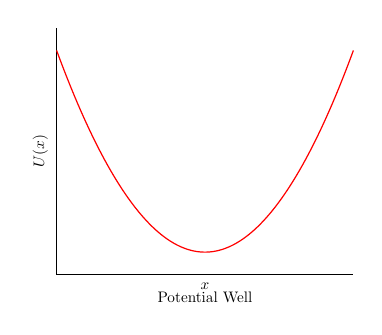
\begin{tikzpicture}[scale=0.55]
            \begin{axis}[
                axis lines=left,
                xlabel=$x$,
                ylabel=$U(x)$,
                ymin=-1, ymax=10,
                xtick=\empty, ytick=\empty,
                axis line style={-},
                clip=false
            ]
            \addplot [
                domain=-3:3,
                samples=100,
                color=red,
                thick,
            ]
            {x^2};
            \node at (axis cs:0, -2) {Potential Well};
            \end{axis}
        \end{tikzpicture}
        \end{minipage}
        \begin{minipage}{0.4\textwidth}    
        \begin{tikzpicture}[scale=0.55]
            \begin{axis}[
                axis lines=left,
                xlabel=$x$,
                ylabel=$P(x)$,
                ymin=0, ymax=1.25,
                xtick=\empty, ytick=\empty,
                axis line style={-},
                clip=false
            ]
            \addplot [
                domain=-3:3,
                samples=100,
                color=blue,
                thick,
            ]
            {exp(-x^2)};
            \node at (axis cs:0, -0.25) {Stationary PDF};
            \end{axis}
        \end{tikzpicture}
        \end{minipage}
    \end{center}
    \end{exampleblock}

\subsection{Special Cases of the Fokker-Planck Equation}

\subsubsection{Deterministic Systems with Random Initial Conditions}
Suppose we have a deterministic system, $\dot{x} = a(x)$, but where the initial conditions are described by a probability distribution $\theta(x)$. Here, randomness comes only from the initial condition, not from noise in the dynamics: the diffusion coefficient is zero, $b(x)=0$. The Fokker-Planck equation loses its second-order derivative term and becomes the \textbf{Liouville equation}:
\small
$$
\begin{cases}
    \dfrac{\partial P(x,t)}{\partial t} = -\dfrac{\partial}{\partial x}\left(a(x)P(x,t)\right) \\[0.8em]
    P(x,0) = \theta(x)
\end{cases}
$$
\normalsize
This type of problem appears, for example, when studying the evolution of a population's distribution over time under deterministic laws, but starting from a known initial distribution.

\subsubsection{Purely Diffusive Systems}
The opposite case occurs when $a(x)=0$, and the system is governed only by noise:
$$
dx = b(x)dW
$$
In population dynamics, this is useful in cases where the baseline growth rate is zero ($r=0$) or constant. In this situation, the Fokker-Planck equation becomes a pure diffusion equation:
$$
\partial_t P = \partial_x^2 \left( \frac{b(x)^2}{2} P(x,t) \right)
$$
This is, in fact, a generalization of the process for the Wiener process, which I recall is $\dot{w} = \xi(t)$ (i.e., $a=0, b=1$). Indeed, using the Fokker-Planck equation, we can find the expression for the PDF of the Wiener process, which will be:
$$
\partial_t P = \frac{1}{2} \partial_w^2 P
$$
Or, analogously, for $\dot{x} = \omega\xi(t)$, which corresponds to the overdamped Brownian motion:
$$
\partial_t P = \frac{\omega^2}{2} \partial_x^2 P
$$

\subsubsection{The Probability Current}
The Fokker-Planck equation can also be viewed in a different way. Given the formula:
\small
$$
\partial_t P = \partial_x \left[ -a(x)P(x,t) - \partial_x \left( \frac{b(x)^2}{2}P(x,t) \right) \right]
$$
\normalsize
If we pull the outer $\partial_x$ out and name the term inside the square brackets $J$, we get:
$$
\partial_t P + \partial_x J = 0
$$
which is the continuity (or flux) equation; in the multi-dimensional case, it is typically written as:
$$
\partial_t \eta + \nabla \cdot J = 0
$$
This makes intuitive sense: if we think of probability as a "substance" (like a population density $\eta$), the change in its distribution is nothing more than a redistribution, so the total amount does not change. The 1D equation found above is easily reduced from the multi-D form of the flux equation. If we take Brownian motion as an example, then:
$$
J = -K \nabla P
$$
For this reason, $J$ in these cases is also known as the \textbf{current}.

\subsubsection{Kac's Lemma} \label{sec:kac}

Kac's Lemma establishes a fundamental relationship between stationary probabilities and expected return times in ergodic stochastic processes. Consider a stationary Markov process with stationary distribution $\pi$ and let $A$ be a measurable subset of the state space. Define $T_A$ as the first return time to $A$ when starting from a point in $A$. Kac's Lemma states:

$$
\mathbb{E}[T_A | X_0 \in A] = \frac{1}{\pi(A)}
$$

where $\pi(A) = \int_A \pi(x) dx$ is the stationary measure of set $A$.

This result provides a direct connection between the equilibrium properties of the system (captured by $\pi$) and its dynamical properties (captured by return times). States or regions with low stationary probability have correspondingly long expected return times.

The lemma follows from the ergodic theorem: for an ergodic process, the long-run proportion of time spent in any set equals its stationary probability. Since visits to $A$ occur approximately every $\mathbb{E}[T_A]$ time units, we have $\pi(A) \approx 1/\mathbb{E}[T_A]$.

This relationship has important applications in population dynamics, where rare population states correspond to long recovery times, and in statistical mechanics, where it connects equilibrium distributions to relaxation timescales near phase transitions.

\section{The Ornstein-Uhlenbeck Process}

We now consider one of the most important stochastic processes in science and engineering: the \textbf{Ornstein-Uhlenbeck (OU) process}. It appears in numerous contexts, from describing the velocity of a particle in a fluid (the original Langevin model) to modeling the voltage in a noisy electronic circuit. In essence, it is the canonical model for any noisy, linear system that tends to return to an equilibrium state.

The general form of the OU process is given by the SDE:
$$
dz = -\gamma z\,dt + \omega\,dW
$$
where $\gamma > 0$ is the \textit{drift} or \textit{relaxation rate}, which constantly pulls the process back towards its mean (in this case, zero), and $\omega$ is the noise intensity. This linear restoring force is what distinguishes the OU process from the free-wandering Wiener process.

\subsubsection{Solving the Ornstein-Uhlenbeck SDE}

To solve this linear SDE, we can use a technique analogous to the integrating factor method for ODEs. We define a new variable $Q(t) = e^{\gamma t}z(t)$. Our goal is to find an SDE for $Q(t)$. Using Ito's product rule (or Ito's lemma on $\psi(z,t) = e^{\gamma t}z$), we find:
\begin{align*}
    dQ &= (d(e^{\gamma t}))z + e^{\gamma t}(dz) \\
    &= (\gamma e^{\gamma t}dt)z + e^{\gamma t}(-\gamma z\,dt + \omega dW(\tau)) \\
    &= \gamma e^{\gamma t}z\,dt - \gamma e^{\gamma t}z\,dt + \omega e^{\gamma t}dW(\tau) \\
    &= \omega e^{\gamma t}dW(\tau)
\end{align*}
The drift terms have canceled perfectly, leaving a very simple SDE for $Q(t)$. We can now integrate it from 0 to $t$:
$$
Q(t) - Q(0) = \omega \int_0^t e^{\gamma \tau}dW(\tau) \quad \implies \quad Q(t) = Q(0) + \omega \int_0^t e^{\gamma \tau}dW(\tau)
$$
Substituting back $z(t) = e^{-\gamma t}Q(t)$ and $z(0) = Q(0)$, we arrive at the solution for the Ornstein-Uhlenbeck process:
$$
z(t) = z(0)e^{-\gamma t} + \omega \int_0^t e^{\gamma(\tau-t)}dW(\tau)
$$
The solution consists of two parts: a deterministic decay of the initial condition, $z(0)e^{-\gamma t}$, and a stochastic integral that represents the accumulated effect of the noise, with past noise contributions being exponentially "forgotten" over time due to the $e^{\gamma(\tau-t)}$ term.

\subsubsection{Statistical Properties}

From the solution, we can derive the key statistical properties of the OU process.

\begin{itemize}
    \item \textbf{Mean}

    Since the stochastic integral $\int e^{\gamma(\tau-t)}dW(\tau)$ has zero mean, the mean of the process is simply the deterministic part:
    $$
    \boxed{\langle z(t) \rangle = \langle z(0) \rangle e^{-\gamma t}}
    $$
    Assuming a deterministic starting point $z(0)$, the mean exponentially decays to zero, which is the equilibrium point of the system.

    \item \textbf{Variance}
    
    The variance calculation is more involved but highly instructive. Starting from our solution:
    $$
    z(t) = z(0)e^{-\gamma t} + \omega \int_0^t e^{\gamma(\tau-t)}dW(\tau)
    $$
    we can calculate the variance by expanding $\text{Var}[z(t)] = \langle z(t)^2 \rangle - \langle z(t) \rangle^2$. Since $\langle z(t) \rangle = z(0)e^{-\gamma t}$ (assuming deterministic initial condition), we have:
    $$
    \text{Var}[z(t)] = \left\langle \left( z(0)e^{-\gamma t} + \omega \int_0^t e^{\gamma(\tau-t)}dW(\tau) \right)^2 \right\rangle - z(0)^2e^{-2\gamma t}
    $$
    Expanding the square:
    \small
    $$
    \text{Var}[z(t)] = \left\langle z(0)^2e^{-2\gamma t} + 2z(0)e^{-\gamma t}\omega \int_0^t e^{\gamma(\tau-t)}dW(\tau) + \omega^2 \left(\int_0^t e^{\gamma(\tau-t)}dW(\tau)\right)^2 \right\rangle - z(0)^2e^{-2\gamma t}
    $$
    \normalsize
    The cross term vanishes since $\langle dW(\tau) \rangle = 0$, leaving:
    $$
    \text{Var}[z(t)] = \omega^2 \left\langle \left(\int_0^t e^{\gamma(\tau-t)}dW(\tau)\right)^2 \right\rangle
    $$
    
    Applying the mean, we get:
    $$
    \text{Var}[z(t)] = \omega^2 \left\langle \left(\int_0^t e^{\gamma(\tau-t)}dW(\tau)\right)^2 \right\rangle = \omega^2 \int_0^t \int_0^t e^{\gamma(\tau-t)}e^{\gamma(s-t)}\langle dW(\tau)dW(s) \rangle
    $$
    Using the property that $\langle dW(\tau)dW(s) \rangle = \delta(\tau - s)d\tau ds$, the double integral becomes:
    $$
    \text{Var}[z(t)] = \omega^2 \int_0^t \int_0^t e^{\gamma(\tau + s -2t)}\delta(s-\tau)\,ds\,d\tau  = \omega^2 \int_0^t e^{2\gamma(\tau-t)}d\tau
    $$
    Evaluating this integral:
    $$
    \text{Var}[z(t)] = \omega^2 e^{-2\gamma t} \int_0^t e^{2\gamma\tau}d\tau = \omega^2 e^{-2\gamma t} \left[ \frac{e^{2\gamma\tau}}{2\gamma} \right]_0^t = \frac{\omega^2}{2\gamma}(1 - e^{-2\gamma t})
    $$

    The total variance becomes:
    $$
    \boxed{\text{Var}[z(t)] = \text{Var}[z(0)]e^{-2\gamma t} + \frac{\omega^2}{2\gamma}(1 - e^{-2\gamma t})}
    $$
    As $t \to \infty$, the first term vanishes, and the variance approaches a constant stationary value:
    $$
    \lim_{t\to\infty} \text{Var}[z(t)] = \frac{\omega^2}{2\gamma}
    $$
    This is a crucial difference from the Wiener process, whose variance grows linearly and without bound. The restoring force in the OU process balances the diffusive effect of the noise, leading to a finite stationary variance.

    \item \textbf{Autocovariance}

    The autocovariance function for times $t$ and $q$ is defined as:
    $$
    C(t,q) = \langle (z(t) - \langle z(t) \rangle)(z(q) - \langle z(q) \rangle) \rangle
    $$
    For simplicity, let's assume the process starts at $z(0) = 0$. In this case, the mean is $\langle z(t) \rangle = 0$ for all $t$, so the autocovariance is simply the autocorrelation: $C(t,q) = \langle z(t)z(q) \rangle$.

    Using the solution for $z(t)$ with $z(0)=0$:
    $$
    z(t) = \omega \int_0^t e^{\gamma(s-t)}dW(s)
    $$
    The autocorrelation is:
    \small
    \begin{align*}
        \langle z(t)z(q) \rangle &= \left\langle \left( \omega \int_0^t e^{\gamma(s-t)}dW(s) \right) \left( \omega \int_0^q e^{\gamma(\tau-q)}dW(\tau) \right) \right\rangle \\
        &= \omega^2 e^{-\gamma(t+q)} \left\langle \int_0^t e^{\gamma s}dW(s) \int_0^q e^{\gamma \tau}dW(\tau) \right\rangle \\
        &= \omega^2 e^{-\gamma(t+q)} \int_0^t \int_0^q e^{\gamma(s+\tau)} \langle dW(s)dW(\tau) \rangle
    \end{align*}
    \normalsize
    Using the property $\langle dW(s)dW(\tau) \rangle = \delta(s-\tau)ds\,d\tau$, the double integral collapses into a single integral. We must evaluate the integral over the domain $[0,t] \times [0,q]$.
    $$
    \langle z(t)z(q) \rangle = \omega^2 e^{-\gamma(t+q)} \int_0^t \int_0^q \, e^{\gamma(\tau + s)} \delta(\tau - s) d\tau ds
    $$
    
For the evaluation of this integral, we need to consider two cases:

    \begin{itemize}
        \item \textbf{Case 1: $t \leq q$}
        
        When $t \leq q$, the domain of integration is restricted by the smaller upper limit. The delta function $\delta(\tau - s)$ forces $\tau = s$, so we integrate over the overlap region $[0, t]$:
        $$
        \langle z(t)z(q) \rangle = \omega^2 e^{-\gamma(t+q)} \int_0^t e^{2\gamma s} ds
        $$

        \vspace{-0.5em}

        Evaluating the integral:
        $$
        \langle z(t)z(q) \rangle = \omega^2 e^{-\gamma(t+q)} \left[ \frac{e^{2\gamma s}}{2\gamma} \right]_0^t = \frac{\omega^2}{2\gamma} e^{-\gamma(t+q)} (e^{2\gamma t} - 1)
        = \frac{\omega^2}{2\gamma} \left( e^{-\gamma(q-t)} - e^{-\gamma(q+t)} \right)
        $$

        \item \textbf{Case 2: $t > q$}
        
        When $t > q$, we integrate over $[0, q]$:
        $$
        \langle z(t)z(q) \rangle = \omega^2 e^{-\gamma(t+q)} \int_0^q e^{2\gamma s} ds = \frac{\omega^2}{2\gamma} \left( e^{-\gamma(t-q)} - e^{-\gamma(t+q)} \right)
        $$
    \end{itemize}

    Combining both cases, we can write the autocorrelation function as:
    $$
    \boxed{\langle z(t)z(q) \rangle = \frac{\omega^2}{2\gamma} \left( e^{-\gamma|t-q|} - e^{-\gamma(t+q)} \right)}
    $$
    For a stationary process (when $t, q \to \infty$), the second term vanishes, and we obtain the stationary autocorrelation function:
    $$
    R_z(\tau) = \lim_{t \to \infty} \langle z(t)z(t + \tau) \rangle = \frac{\omega^2}{2\gamma} e^{-\gamma|\tau|}
    $$
    where $\tau = |t-q|$ is the time lag. This autocorrelation decays exponentially with a characteristic time $1/\gamma$. In the limit of rapid relaxation ($\gamma \to \infty$), the autocorrelation function becomes sharply peaked and tends toward a Dirac delta function.
\end{itemize}

We introduce now a scaling relation between the noise intensity and the relaxation rate, by setting:
$$
\omega = c\,\gamma
$$
with $c$ a constant. Under this scaling, the SDE for $z$ becomes
$$
\dot{z} = -\gamma\,z + c\,\gamma\,\xi(t).
$$

The autocorrelation function for $z$ then reads
$$
R_z(h) = \frac{c^2}{2}\,\gamma\,e^{-\gamma|h|}, \qquad R_z(0) = \frac{c^2}{2}\,\gamma.
$$
Its total area is given by
$$
\int_{-\infty}^{+\infty} R_z(h)\,dh 
=
\int_{-\infty}^{+\infty} \frac{c^2}{2}\,\gamma\,e^{-\gamma|h|}\,dh.
=
\frac{c^2}{2}\,\gamma \cdot \frac{2}{\gamma} = c^2.
$$

For small characteristic times ($\tau=1/\gamma$ small), the autocorrelation function $R_z(h)$ approximates a white noise process:
$$
\lim_{\gamma \to \infty} R_z(h;\gamma) = c^2\,\delta(h).
$$

This derivation shows how, by choosing the scaling $\omega = c\,\gamma$, the fluctuations in the linearized dynamics around a stable equilibrium effectively become white noise in the fast relaxation limit.

\subsection{The OU Process as a Low-Pass Filter}

One of the most important interpretations of the Ornstein-Uhlenbeck process is as a \textbf{low-pass filter}. It takes a "noisy" input signal (white noise) and produces a smoother, more physically realistic output by attenuating high-frequency fluctuations. To understand this, we can analyze the process in the frequency domain using the Fourier transform.

\subsubsection{The Fourier Transform and Linear Systems}
Let $f(t)$ be a well-behaved function. Its Fourier transform, $\hat{f}(\omega)$, is defined as:
$$
\mathcal{F}[f(t)] = \hat{f}(\omega) = \int_{-\infty}^{+\infty} f(t) e^{-i\omega t} dt
$$
A key property of the Fourier transform, which can be shown using integration by parts, is how it acts on derivatives:
$$
\mathcal{F}[f'(t)] = i\omega \mathcal{F}[f(t)] = i\omega \hat{f}(\omega)
$$
This property turns differentiation in the time domain into multiplication in the frequency domain, which is extremely useful for solving linear differential equations. For example, consider a general first-order linear system with input $y(t)$ and output $f(t)$:
$$
f'(t) + \alpha f(t) = y(t)
$$
Taking the Fourier transform of the entire equation gives:
$$
i\omega\hat{f}(\omega) + \alpha\hat{f}(\omega) = \hat{y}(\omega) \quad \implies \quad \hat{f}(\omega) = \frac{\hat{y}(\omega)}{i\omega + \alpha}
$$
The term $H(\omega) = 1/(i\omega + \alpha)$ is called the \textbf{transfer function} of the system. The power of the output signal is related to the power of the input signal by the squared magnitude of the transfer function:
$$
|\hat{f}(\omega)|^2 = \frac{|\hat{y}(\omega)|^2}{\omega^2 + \alpha^2}
$$

\subsubsection{Power Spectrum of the OU Process}
We can apply this framework to the OU process, which is described by the linear SDE:
$$
\frac{dz}{dt} + \gamma z = \kappa \xi(t)
$$
Taking the Fourier transform, we get:
$$
(i\omega + \gamma)\hat{z}(\omega) = \kappa \mathcal{F}[\xi(t)] \quad \implies \quad \hat{z}(\omega) = \frac{\kappa}{i\omega + \gamma} \mathcal{F}[\xi(t)]
$$
To analyze the filtering effect, we compare the \textbf{power spectral density} of the input signal, $\xi(t)$, with that of the output signal, $z(t)$. The power spectrum is the Fourier transform of the autocorrelation function.

For the input signal (white noise), the autocorrelation is $R_{\xi}(h) = \delta(h)$ (assuming unit variance for simplicity). Its power spectrum is therefore constant:
$$
\mathcal{F}[R_{\xi}(h)] = \mathcal{F}[\delta(h)] = \int_{-\infty}^{+\infty} \delta(h) e^{-i\omega h} dh = 1
$$
This flat spectrum is why it's called "white" noise: it contains equal power at all frequencies $\omega$.

For the output signal, $z(t)$, we previously found its stationary autocorrelation function to be:
$$
R_{z}(h) = \frac{\kappa^2}{2\gamma} e^{-\gamma|h|}
$$
The power spectrum of the output is the Fourier transform of this function:
$$
\mathcal{F}[R_{z}(h)] = \frac{\kappa^2}{2\gamma} \int_{-\infty}^{+\infty} e^{-\gamma|h|} e^{-i\omega h} dh
$$
We can split the integral over positive and negative values of $h$:
$$
= \int_{-\infty}^{0} e^{(\gamma-i\omega)h}dh + \int_{0}^{+\infty} e^{-(\gamma+i\omega)h}dh = \frac{1}{\gamma-i\omega} + \frac{1}{\gamma+i\omega} = \frac{2\gamma}{\gamma^2 + \omega^2}
$$
Substituting this back, we get the output power spectrum:
$$
\mathcal{F}[R_{z}(h)] = \frac{\kappa^2}{2\gamma} \left( \frac{2\gamma}{\gamma^2 + \omega^2} \right) = \frac{\kappa^2}{\gamma^2 + \omega^2}
$$
This function, known as a \textbf{Lorentzian}, is peaked at $\omega=0$ and decays as $1/\omega^2$ for high frequencies. The OU process acts as a low-pass filter: it suppresses high-frequency components of the input white noise while allowing low-frequency components to pass through, resulting in a smoother, more physically plausible random process.

\vspace{-0.5em}
\begin{figure}[H]
    \centering
    \begin{minipage}{0.45\textwidth}
    \centering
    % Input graph: a constant function
    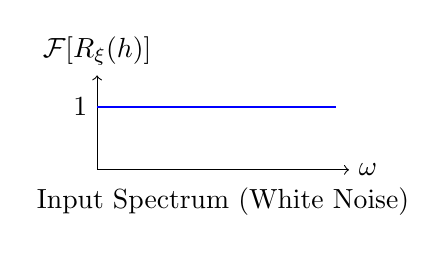
\begin{tikzpicture}[scale=0.8]
        \draw[->] (0,0) -- (4,0) node[right] {$\omega$};
        \draw[->] (0,0) -- (0,1.5) node[above] {$\mathcal{F}[R_{\xi}(h)]$};
        \draw[blue, thick] (0,1) -- (3.8,1) node[right] {};
        \node at (0,1) [left] {$1$};
        \node at (2,-0.5) {Input Spectrum (White Noise)};
    \end{tikzpicture}
    \end{minipage}
    \hfill
    \begin{minipage}{0.45\textwidth}
    \centering
    % Output graph: a Lorentzian shape
    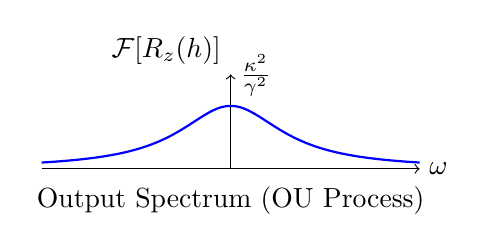
\begin{tikzpicture}[scale=0.8]
        \draw[->] (-3,0) -- (3,0) node[right] {$\omega$};
        \draw[->] (0,0) -- (0,1.5) node[above left] {$\mathcal{F}[R_{z}(h)]$};
        \draw[blue, thick, domain=-3:3, samples=100] plot (\x,{1/(1+\x*\x)});
        \node at (0,1) [above right] {$\frac{\kappa^2}{\gamma^2}$};
        \node at (0,-0.5) {Output Spectrum (OU Process)};
    \end{tikzpicture}
    \end{minipage}
    \caption{Power spectra: input white noise (flat, left) and output OU process (Lorentzian, right).}
\end{figure}

\vspace{-1em}

\subsection{Fokker-Planck equation for Ornstein-Uhlenbeck}

Given the Ito equation for the OU process:
$$
    dz = -\gamma z dt + \omega dW
$$
we can find the Fokker-Planck equation. Recalling the general form of the equation for $P(z,t)$:
$$
    \partial_t P = -\partial_z[a(z)P(z,t)] + \frac{1}{2} \partial_z^2 \left[ b(z)^2 P(z,t) \right]
$$
In our case, with $a(z) = -\gamma z$ and $b(z) = \omega$, it becomes:
$$
    \partial_t P = \partial_z(\gamma z P) + \frac{\omega^2}{2} \partial_z^2 P
$$
This equation is not simple to solve, even with the boundary conditions for a probability density:
$$
    P(\pm\infty, t) = 0 \quad \text{and} \quad \int_{\mathbb{R}} P(z, t) dz = 1
$$
These are additional conditions compared to standard PDEs and are usually of great help.

The most tractable approach is to find the stationary solution $P_s(z)$, which is the long-time limit of $P(z,t)$:
$$
    P_s(z) = \lim_{t\to\infty} P(z,t)
$$
In the stationary state, $\partial_t P = 0$, so the equation becomes an ODE:
$$
    0 = \frac{d}{dz}(\gamma z P_s) + \frac{\omega^2}{2} \frac{d^2 P_s}{d z^2}
$$
which we can rearrange to:
$$
    \frac{d^2 P_s}{d z^2} = - \frac{2\gamma}{\omega^2} \frac{d}{dz}(z P_s)
$$
Integrating once with respect to $z$, we obtain:
$$
    \frac{d P_s}{dz} = C - \frac{2\gamma}{\omega^2} z P_s(z)
$$
The boundary conditions require that $P_s(z) \to 0$ and consequently $P_s'(z) \to 0$ as $z \to \pm\infty$. For this to hold, the integration constant $C$ must be zero. This leaves us with a first-order linear ODE:
$$
    \frac{dP_s}{dz} = - \frac{2\gamma}{\omega^2} z P_s(z)
$$
The solution is a Gaussian function, which is consistent with the properties of the Ornstein-Uhlenbeck process:
$$
    P_s(z) = A e^{-\frac{\gamma}{\omega^2}z^2}
$$
This is nothing other than a Gaussian with $\mu = 0$ and $\sigma^2 = \omega^2/2\gamma$, with $A$ a constant required for normalization, namely
$$
A = \frac{1}{\sqrt{2\pi\sigma^2}}
$$

If we now consider the unperturbed system $\dot{z} = -\gamma z$, we see that the solution tends to $0$ for long times and, since it is deterministic, we obviously have
$$
P^{\mathrm{DET}}_s(z) = \delta(z)
$$
which is consistent with the perturbed case. In fact, the only equilibrium point of the deterministic case is $0$, which turns out to be the center of the Gaussian we found. Therefore, for long times, in the perturbed case, the solution will oscillate around $0$.

\section{The Ginzburg-Landau Model}

We now move from the monostable Ornstein-Uhlenbeck process to a more complex and interesting class of systems: bistable systems. These are systems that possess two stable equilibrium states. The simplest and most iconic model for such a system is the \textbf{Ginzburg-Landau equation}.

\subsubsection{The Deterministic Model}

The deterministic Ginzburg-Landau model describes the dynamics of a particle in a "double-well" potential. The equation of motion is given by:
$$
\dot{x} = x - x^3 = x(1-x)(1+x)
$$
This system has three equilibrium points, found by setting $\dot{x} = 0$:
$$
x_L = -1, \quad x_C = 0, \quad x_R = +1
$$
A simple stability analysis reveals the nature of these points:
\begin{itemize}
    \item $x_L = -1$ and $x_R = +1$ are \textbf{locally asymptotically stable}. If the system starts near one of these points, it will converge to it.
    \item $x_C = 0$ is an \textbf{unstable} equilibrium. If the system starts at this point, any infinitesimal perturbation will cause it to move away towards either $x_L$ or $x_R$.
\end{itemize}

The force $F(x) = x - x^3$ can be derived from a potential $U(x)$ where $F = -dU/dx$:
$$
U(x) = -\frac{x^2}{2} + \frac{x^4}{4}
$$
This potential has a characteristic "double-well" shape, where the stable equilibria $x_L$ and $x_R$ correspond to the minima (the "wells") of the potential, and the unstable equilibrium $x_C=0$ corresponds to the local maximum (the "barrier") between them.

If the initial condition $x(0)$ is drawn from a probability distribution $\theta(x)$, the long-term behavior of the system is deterministic. Any trajectory with $x(0) > 0$ will end up at $x_R = +1$, and any with $x(0) < 0$ will end up at $x_L = -1$. The stationary PDF will therefore consist of two Dirac delta peaks at the stable equilibria, with weights determined by the initial probability of being on either side of the unstable point:
$$
\lim_{t\to\infty} \rho(x,t) = A_R \delta(x-1) + A_L \delta(x+1)
$$
where $A_R = \text{Pr}(x_0>0)$ and $A_L = \text{Pr}(x_0<0)$.

\subsubsection{Stochastic Perturbations of the Model}

Now, let's add a stochastic white noise force to the system:
$$
\dot{x} = x - x^3 + \omega\xi(t) \quad \text{or} \quad dx = (x-x^3)dt + \omega dW_t
$$
This is a case of additive noise perturbing a conservative force. As we derived previously, the stationary probability distribution $P_s(x)$ for such a system is given by the Boltzmann distribution:
$$
P_s(x) = C \exp\left(-\frac{2}{\omega^2}U(x)\right)
$$
Substituting the Ginzburg-Landau potential $U(x) = -x^2/2 + x^4/4$, we get:
$$
P_s(x) = C \exp\left(-\frac{2}{\omega^2}\left(-\frac{x^2}{2} + \frac{x^4}{4}\right)\right) = C \exp\left(\frac{x^2}{\omega^2} - \frac{x^4}{2\omega^2}\right)
$$
where $C$ is a normalization constant. The shape of this distribution is fundamentally controlled by the noise intensity $\omega$.

% picture ?

The relationship between the potential $U(x)$ and the stationary PDF $P_s(x)$ is clear:
\begin{itemize}
    \item The stable equilibria of the deterministic system (minima of $U(x)$) become the \textbf{modes} (peaks) of the stationary PDF.
    \item The unstable equilibrium (maximum of $U(x)$) becomes the \textbf{antimode} (trough) of the stationary PDF.
\end{itemize}

The noise intensity $\omega$ determines how closely the system is confined to these potential wells:
\begin{itemize}
    \item \textbf{Weak Noise ($\omega \ll 1$):} The distribution $P_s(x)$ is sharply bimodal, with two distinct peaks centered around $x=-1$ and $x=+1$. The probability of finding the particle near the unstable point $x=0$ is extremely low. The system will exhibit small stochastic fluctuations around one of the two stable states for very long periods.
    \item \textbf{Strong Noise ($\omega \gg 1$):} The noise provides enough energy for the particle to easily cross the potential barrier between the two wells. The two peaks in the PDF broaden and merge, and the distribution becomes unimodal, centered at $x=0$. For very large $x$, the $x^4$ term still dominates, so the probability $P_s(x)$ must decay to zero.
\end{itemize}

\begin{minipage}{0.48\textwidth}
    \begin{figure}[H]
    \centering
    % PDF for small omega
    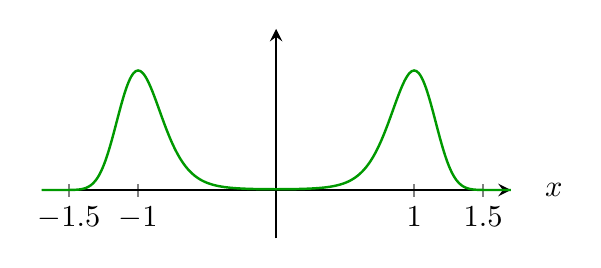
\begin{tikzpicture}[scale=1.1]
        \begin{axis}[
            width=7cm,
            height=4cm,
            domain=-1.7:1.7,
            samples=200,
            axis lines=middle,
            xlabel={$x$},
            ylabel={},
            xtick={-1.5,-1,0,1,1.5},
            ytick=\empty,
            ymin=-60, ymax=200,
            xmin=-1.7, xmax=1.7,
            every axis y label/.style={at={(ticklabel* cs:1.05)},anchor=south},
            every axis x label/.style={at={(ticklabel* cs:1.05)},anchor=west},
            axis line style=thick,
            tick style={thick}
        ]
        % Small omega: sharply bimodal
        \addplot[domain=-1.7:1.7, smooth, thick, color=green!60!black] {exp(x^2/0.1 - x^4/0.2)};
        \end{axis}
    \end{tikzpicture}
    \caption{PDF (non normalized) for small $\omega$}
    \end{figure}
\end{minipage}
\hfill
\begin{minipage}{0.48\textwidth}
    \begin{figure}[H]
    \centering
    % PDF for large omega
    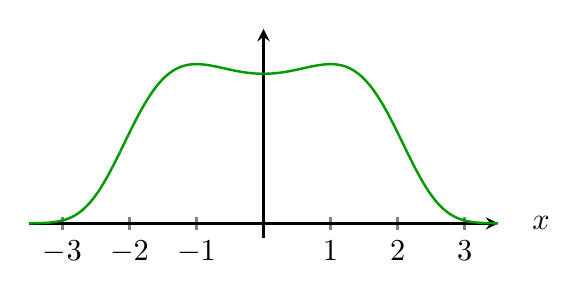
\begin{tikzpicture}[scale=1.1]
        \begin{axis}[
            width=7cm,
            height=4cm,
            domain=-3.5:3.5,
            samples=200,
            axis lines=middle,
            xlabel={$x$},
            ylabel={},
            xtick={-3,-2,-1,0,1,2,3},
            ytick=\empty,
            ymin=-0.1, ymax=1.3,
            xmin=-3.5, xmax=3.5,
            every axis y label/.style={at={(ticklabel* cs:1.05)},anchor=south},
            every axis x label/.style={at={(ticklabel* cs:1.05)},anchor=west},
            axis line style=thick,
            tick style={thick}
        ]
        % Large omega: broad, unimodal
        \addplot[domain=-3.5:3.5, smooth, thick, color=green!60!black] {exp(x^2/8 - x^4/16)};
        \end{axis}
    \end{tikzpicture}
    \caption{PDF (non normalized) for large $\omega$}
    \end{figure}
\end{minipage}

\vspace{0.5em}

This "inheritance" of stability properties from the deterministic potential to the modes of the stationary PDF is a key feature of systems with additive noise. As we will see, this direct correspondence breaks down in the presence of multiplicative noise.

\begin{observationblock}[Stochastic Miultistability]
    It is possible to say that after a very long period of time, also the first case we could see that the system moves from one peak to the other. This is due to the fact that the system is not stable and we have a non-zero probability of moving from one peak to the other. 
\end{observationblock}

\section{Multiplicative Noise}

While additive noise provides a good model for systems perturbed by external forces, many real-world systems feature fluctuations whose intensity depends on the state of the system itself. This leads to the concept of \textbf{multiplicative noise}, which can induce much richer and more complex behaviors than its additive counterpart.

\subsubsection{General SDE and Stationary Fokker-Planck Equation}

Consider a system governed by a parameter $p$. The simplest case is when it is possible to write the field in the form
$$
\dot{x} = b(x) + p \hat{g}(x)
$$
that is, with linear dependence on the parameter considered. The parameter $p$ is usually influenced by the external world, so in some cases it is possible for it to become stochastic. We can then describe a stochastic $p$ as
$$
p \to p + \alpha \xi(t)
$$
Substituting, we obtain
$$
\dot{x} = b(x) + p \hat{g}(x) + \hat{g}(x) \alpha \xi(t)
$$
We can then group the stochastic terms, obtaining
$$
\dot{x} = f(x) + g(x) \xi(t)
$$
The Fokker-Planck equation for the general case is:
$$
\frac{\partial \rho}{\partial t} = - \frac{\partial}{\partial x} [f(x) \rho] + \frac{\partial^2}{\partial x^2} \left[ \frac{g(x)^2}{2} \rho \right]
$$
So far, we have only considered cases where $g(x)$ is constant. Here, however, we are dealing with the most general version of what we have seen so far. The boundary conditions remain the same as before, and as usual, we analyze the stationary case. We have:
$$
\frac{d}{dx} \left[ \frac{g(x)^2}{2} P_s(x) \right] = f(x)P_s(x)
$$
This is a first-order ODE that can be solved for $P_s(x)$. Let's define an auxiliary function $Q(x) = \frac{g(x)^2}{2} P_s(x)$. The equation becomes:
$$
\frac{dQ}{dx} = f(x) \frac{2}{g(x)^2} Q(x)
$$
This is a standard linear ODE of the form $Q'(x) = a(x)Q(x)$, whose solution is $Q(x) = C e^{A(x)}$, where $A(x) = \int a(s)ds$. Applying this, we find:
$$
Q(x) = C \exp\left( \int \frac{2f(s)}{g(s)^2} ds \right)
$$
Substituting back $P_s(x) = \frac{2}{g(x)^2}Q(x)$, we arrive at the general solution for the stationary PDF:
$$
P_s(x) = \frac{C'}{g(x)^2} \exp\left( \int^x \frac{2f(z)}{g(z)^2} dz \right)
$$
where $C'$ is a normalization constant. Let's remark that, being a probability density, the integral of $P_s(x)$ over the entire state space must be equal to one.

We can distinguish two cases:
\begin{itemize}
    \item If the integral exists (is finite), then everything is fine and we can calculate $C$ to normalize $P_s(x)$.
    \item If instead the integral is infinite, we can only find a formal solution that has no physical meaning: in this case it is necessary to study the steady state directly starting from the SDE.
\end{itemize}

\subsection{Noise-Induced Transitions}

In the case of additive noise ($g(x) = \text{const}$), the extrema of the stationary PDF $P_s(x)$ coincide with the equilibria of the deterministic system (where $f(x)=0$). With multiplicative noise, this simple correspondence breaks down.

Recall the following identity, which will be useful for manipulating the stationary distribution:
$$
\dfrac 1{g^2(x)} = e^{-\ln g^2(x)} = e^{-2 \ln g(x)}
$$

Using this, we can rewrite the stationary probability density function in a more transparent exponential form:
$$
P_s(x) = 2 C \exp \left\{
    - 2 \log (g(x)) + \int_\alpha^x \dfrac{2 f(s)}{g^2(s)} ds
\right\}
$$
This highlights how both the noise amplitude $g(x)$ and the drift $f(x)$ contribute to shaping the stationary distribution.

To investigate the location of the extrema of $P_s(x)$, we differentiate with respect to $x$. Applying the chain rule to the exponent, we obtain:
$$
P_s'(x) = 2 C \exp \left\{
    - 2 \dfrac{g'(x)}{g(x)} + \dfrac{2 f(x)}{g^2(x)}
    \right\}
$$
This expression will allow us to determine where the stationary distribution attains its maxima and minima, as these correspond to the points where $P_s'(x) = 0$.

To find the extrema of $P_s(x)$, we must find where its derivative is zero, $P_s'(x)=0$. After some algebraic manipulation of the general solution, this condition simplifies to:

$$
f(x) \ge g(x)g'(x)
$$

This time, unfortunately, we no longer have the close connection we had before; everything now depends on $\alpha$ and on the structure of $g(x)$. In fact, I can rewrite the relation as

$$
f(x) \geq \alpha^2 g'(x) g(x)
$$

This remarkable result shows that the modes of the stationary distribution are no longer located at the deterministic equilibria ($f(x)=0$). Instead, their locations are shifted by a term that depends on the noise function $g(x)$ and its derivative.


This phenomenon, discovered by Horsthemke and Lefever in the 1970s, is called a \textbf{Noise-Induced Transition (NIT)}. It means that by simply varying a parameter that controls the noise intensity, new extrema can appear in the PDF that were completely absent in the unperturbed deterministic system.

Before the discovery of NITs, it was commonly believed that noise could only act in two ways:
\begin{itemize}
    \item In unimodal systems, it creates a "cloud" of fluctuations around the single deterministic equilibrium.
    \item In multimodal systems, it can cause "jumps" between the existing deterministic equilibria.
\end{itemize}
NITs showed that noise can play a much more constructive role, inducing oscillations and creating entirely new states that are not present in the unperturbed deterministic system.

\begin{exampleblock}[Noise-Induced Bifurcation in Gene Expression]
Consider a simple model for protein production, where a protein X acts as its own transcription factor. The production rate is $Q(x)$ and the degradation rate is $dx$.
$$
\dot{x} = Q(x) - dx
$$
A common form for $Q(x)$ that models self-regulation is:
$$
Q(x) = R + K\frac{x^2}{K_d + x^2}
$$
where $R$ is a basal production rate and the second term is a Hill function describing feedback. The deterministic system is:
$$
\dot{x} = \underbrace{R + K\frac{x^2}{K_d + x^2} - dx}_{f(x)}
$$
For small degradation rates $d$, this system has a single, globally stable equilibrium point.

Now, suppose the degradation rate $d$ is subject to stochastic fluctuations: $d \to d + \alpha\xi(t)$. The SDE becomes:
$$
dx = \left(R + K\frac{x^2}{K_d + x^2} - dx\right)dt - \alpha x dW_t
$$
Here, the noise is multiplicative, with $g(x) = -\alpha x$, so $g'(x) = -\alpha$. The condition for the extrema of the stationary PDF, $f(x) \ge g(x)g'(x)$, is:
$$
R + K\frac{x^2}{K_d + x^2} - dx \ge (-\alpha x)(-\alpha) = \alpha^2 x
$$
Rearranging gives:
$$
R + K\frac{x^2}{K_d + x^2} \ge (d + \alpha^2)x
$$
Depending on the value of the noise parameter $\alpha$, this algebraic equation can have one or three solutions. This means that by changing the noise intensity, the stationary PDF can transition from being unimodal (with one peak) to bimodal (with two peaks), even though the underlying deterministic system only had one equilibrium point. This is a classic example of a noise-induced transition: the noise itself creates new, stable macroscopic states for the system.
\end{exampleblock}

\newpage

\section{Perturbation of the Logistic Growth Model}
Let's revisit the logistic growth model, which serves as another prime example of how multiplicative noise can fundamentally alter a system's behavior. We start with the deterministic logistic equation:
$$
\dot{z} = r_1 z - r_2 z^2
$$
Through a linear change of variables $x = r_2 z$, we can adimensionalize the equation to a simpler form:
$$
\dot{x} = r x - x^2
$$
Now, we introduce stochasticity by perturbing the intrinsic growth rate, $r \to r + \omega\xi(t)$. This leads to the corresponding Itô equation with multiplicative noise:
$$
dx = (r x - x^2)dt + \omega x dW_t
$$
This defines our drift and diffusion coefficients as $f(x) = r x - x^2$ and $g(x) = \omega x$.

The stationary Fokker-Planck equation for this system is:
$$
\frac{d}{dx} \left[ \frac{g(x)^2}{2} P_s(x) \right] = f(x)P_s(x)
$$
Substituting our specific $f(x)$ and $g(x)$ gives:
$$
\frac{d}{dx} \left[ \frac{\omega^2 x^2}{2} P_s(x) \right] = (r x - x^2)P_s(x)
$$

To solve this differential equation, we can use the substitution method. Let $Q = x^2 P_s$, then:
$$
Q' = \frac{2r-x}{\omega^2 x} Q
$$
This can be rewritten as:
$$
\frac{dQ}{Q} = \frac{2r-x}{\omega^2 x} dx = \left[\frac{2r}{\omega^2 x} - \frac{1}{\omega^2}\right] dx
$$
Integrating both sides:
$$
\ln Q = \frac{2r}{\omega^2} \ln x - \frac{x}{\omega^2} + C
$$
Taking the exponential:
$$
Q(x) = A \exp\left[\frac{2r}{\omega^2} \ln x - \frac{x}{\omega^2}\right] = A x^{\frac{2r}{\omega^2}} e^{-\frac{x}{\omega^2}}
$$
Since $Q = x^2 P_s$, we obtain:
$$
P_s(x) = \frac{Q(x)}{x^2} = A x^{\frac{2r}{\omega^2}-2} e^{-\frac{x}{\omega^2}}
$$
where $A$ is a normalization constant.


A crucial step is to check whether this candidate solution is a valid, normalizable probability distribution. The integral $\int_0^\infty P_s(x) dx$ must be finite.
$$
\int_0^\infty x^{\frac{2r}{\omega^2}-2} e^{-\frac{2}{\omega^2}x} dx
$$
This is a form of the Gamma function integral, $\int_0^\infty t^{k-1}e^{-t}dt$. For this integral to converge at the lower bound ($x \to 0$), the exponent of $x$ must be greater than -1.
$$
\frac{2r}{\omega^2}-2 > -1 \quad \implies \quad \frac{2r}{\omega^2} > 1 \quad \implies \quad r > \frac{\omega^2}{2}
$$

This is valid only if $r > \omega^2/2$ as we have already seen in the past. If this does not hold, we cannot integrate but what does this actually mean? To understand this, let's return to the SDE:
$$
dx = x(r - x)dt + \omega x dW
$$

Applying now the transformation $y = \psi(x) = \log x$, then $\psi'(x) = x^{-1}$ and $\psi''(x) = -x^{-2}$. Therefore:
$$
dy = \left[\frac{1}{\cancel{x}}x(r - x) - \frac{1}{\cancel{x^2}} \frac{\omega^2 \cancel{x^2}}{2}\right]dt + \omega dW
$$

Therefore, substituting in $y$:
$$
dy = \left[r - \frac{\omega^2}{2} - e^y\right]dt + \omega dW
$$

Integrating then:
$$
y(t) = y_0 + \left(r - \frac{\omega^2}{2}\right)t - \int_0^t e^{y(s)}ds + \omega[W(t) - W(0)]
$$

Notice that the integral term, $-\int_0^t e^{y(s)}ds$, is always negative (since $e^{y(s)} > 0$ for all $s$). 

\begin{itemize}

    \item \textbf{Case 1:} $r < \omega^2/2$

    If $r < \omega^2/2$, the drift term $\left(r - \frac{\omega^2}{2}\right)t$ is negative and dominates for large $t$, while the stochastic term becomes negligible in comparison. As a result, $y(t) \to -\infty$ as $t \to \infty$, which means $x(t) = e^{y(t)} \to 0^+$. In this regime, the probability distribution $P(x, t)$ collapses to a delta function at zero:
$$
    \lim_{t \to \infty} P(x, t) = \delta(x)
$$
This shows that, in this case, the Fokker-Planck equation predicts a stationary solution, but in reality, all probability accumulates at extinction ($x=0$). Thus, the Fokker-Planck approach alone can be misleading for this parameter regime.

    \item \textbf{Case 2:} $r > \omega^2/2$

    On the other hand, when $r > \omega^2/2$, the stationary solution is normalizable and given by:
    $$
        P_s(x) = A x^{\frac{2r}{\omega^2}-2} e^{-\frac{2}{\omega^2}x}
    $$

\end{itemize}


\begin{figure}[H]
    \centering
    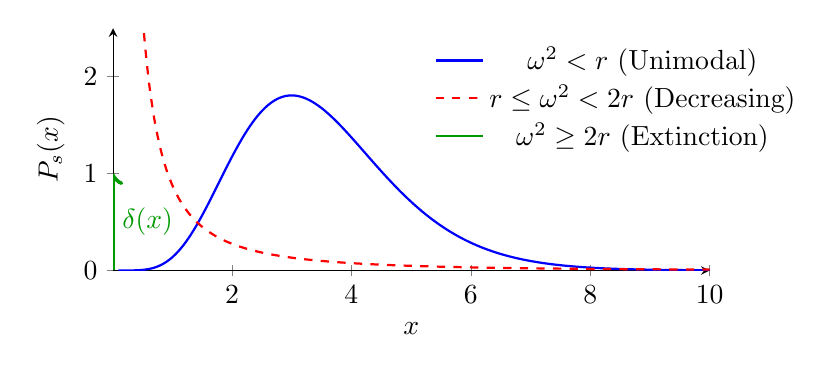
\begin{tikzpicture}
        \begin{axis}[
            scale=0.9,
            width=10cm,
            height=5cm,
            axis lines=left,
            xlabel={$x$},
            ylabel={$P_s(x)$},
            xmin=0.01, xmax=10,
            ymin=0, ymax=2.5,
            legend pos=north east,
            legend style={draw=none, fill=none, xshift=1.5cm},
        ]
        % Case 1: Unimodal PDF (r1 > omega^2)
        \addplot[domain=0.1:10, samples=100, color=blue, thick, smooth] {x^(2*4/1-2)*exp(-2/1*x)};
        \addlegendentry{$\omega^2 < r$ (Unimodal)};
        
        % Case 2: Decreasing PDF (r1 <= omega^2 < 2r1)
        \addplot[domain=0.1:10, samples=100, color=red, thick, smooth, dashed] {x^(2*4/16-2)*exp(-2/16*x)};
        \addlegendentry{$r \le \omega^2 < 2r$ (Decreasing)};
        
        % Case 3: Extinction (delta function, illustrative) - invisible plot for legend
        \addplot[draw=none, color=green!60!black] coordinates {(0,0)};
        \addlegendentry{$\omega^2 \ge 2r$ (Extinction)};
        
        % Case 3: Extinction (delta function, illustrative) - visual representation
        \draw[->, ultra thick, green!60!black] (0.01,0) -- (0.01,1);
        \node[green!60!black, right] at (0, 0.5) {$\delta(x)$};
        
        \end{axis}
    \end{tikzpicture}
    \caption{Noise-Induced Transition in the logistic model.}
\end{figure}


Let us also consider two special cases:
\begin{itemize}
    \item If $\omega^2 = 2r$ (i.e., $2r/\omega^2 = 1$), the stationary distribution simplifies to:
    $$
        P_s(x) = A x^{-1} e^{-\frac{x}{r}}
    $$
    \item If there is no noise, $\omega^2 = 0$, the stationary distribution becomes:
    $$
        P_s(x) = A e^{-\frac{x}{r}}
    $$
    This change has a significant effect on the shape of the stationary distribution. Specifically, when the parameters satisfy
    $$
        \frac{2r}{\omega^2} < 2 \qquad \text{or equivalently} \qquad r < \frac{\omega^2}{2}
    $$
    the distribution $P_s(x)$ is no longer unimodal (with a peak at some $x > 0$), but instead becomes a monotonically decreasing function of $x$. In this regime, the probability density is highest near $x=0$ and decreases for larger $x$, so the system is most likely to be found close to $x=0$.
\end{itemize}


Furthermore, it can be shown that the stationary distribution $P_s(x)$ is normalizable (i.e., its total probability integrates to 1) only if $\omega^2 < 2r$. This is consistent with the more general result discussed in the previous section.

\section{The Stratonovich Integral}

Let us recall that the Itô formula arises from discretizing a stochastic differential equation (SDE) of the form $dx = a(x)dt + b(x)dW_t$ as follows:
$$
x(t+dt) - x(t) = a(x(t))dt + b(x(t))dW_t
$$
In this scheme, the diffusion term $b(x)$ is evaluated at the \emph{start} of the time interval, $t$. This choice is mathematically convenient: it ensures that the integrand does not depend on the future increment $dW_t$, making the resulting stochastic integral a martingale.

However, this is not the only possible convention. An important alternative, introduced by Ruslan Stratonovich, evaluates the diffusion term at the \emph{midpoint} of the interval, $t + dt/2$. This leads to the \textbf{Stratonovich SDE}, which is denoted with a $\circ$:
$$
dx = a(x)dt + b(x) \circ dW_t
$$
The corresponding discretized form is:
$$
x(t+dt) - x(t) = a(x(t))dt + b\left(x\left(t+\frac{dt}{2}\right)\right)dW_t
$$
Although this change in the evaluation point may seem minor, it has significant consequences. The Stratonovich and Itô integrals obey different calculus rules. In particular, while the Itô integral is a martingale, the Stratonovich integral is not. On the other hand, the Stratonovich chain rule matches the familiar rules of ordinary calculus, which often makes it more natural and intuitive for physicists and engineers, especially when modeling systems based on physical laws.

\newpage

\subsubsection{Connecting the Itô and Stratonovich SDEs}
We can find a direct relationship between the two formalisms by expanding the midpoint term in the Stratonovich definition.
First, we approximate the state at the midpoint:
$$
x\left(t+\frac{dt}{2}\right) \approx x(t) + a(x(t))\frac{dt}{2} + b(x(t))\left(W\left(t+\frac{dt}{2}\right) - W(t)\right)
$$
Next, we expand the function $b$ around $x(t)$:
$$
b\left(x\left(t+\frac{dt}{2}\right)\right) \approx b(x(t)) + b'(x(t)) \left( x\left(t+\frac{dt}{2}\right) - x(t) \right)
$$
Substituting the first expression into the second gives:
$$
b\left(x\left(t+\frac{dt}{2}\right)\right) \approx b(x(t)) + b'(x(t))\left[ a(x(t))\frac{dt}{2} + b(x(t))\hat{dW} \right]
$$
where $\hat{dW} = W(t+\frac{dt}{2}) - W(t)$. Now we substitute this back into the Stratonovich SDE definition:
$$
dx = a(x)dt + \left( b(x) + b'(x)\left[ a(x)\frac{dt}{2} + b(x)\hat{dW} \right] \right) dW_t
$$
Expanding this, we get three terms involving $dW_t$:
$$
dx = a(x)dt + b(x)dW_t + a(x)b'(x)\frac{dt}{2}dW_t + b(x)b'(x)\hat{dW}dW_t
$$
The term $dt\,dW_t$ is of order $O(dt^{3/2})$ and can be neglected. The final term requires us to evaluate the expectation $\langle\hat{dW}dW_t\rangle$.
$$
\langle \hat{dW}dW_t \rangle = \left\langle \left(W(t+\frac{dt}{2}) - W(t)\right)\left(W(t+dt) - W(t)\right) \right\rangle = \min\left(t+\frac{dt}{2}, t+dt\right) - t = \frac{dt}{2}
$$
where the minimum comes from the autocorrelation of the Wiener process $\langle W(t)W(s) \rangle = \min(t, s)$.

\vspace{0.5em}

Therefore, the term $b(x)b'(x)\hat{dW}dW_t$ contributes a drift of $\frac{1}{2}b(x)b'(x)dt$.
Combining all terms, the Stratonovich SDE is equivalent to the following Itô SDE:
$$
dx = \left( a(x) + \frac{1}{2}b(x)b'(x) \right)dt + b(x)dW_t
$$

\begin{definitionblock}[Stratonovich-to-Itô Conversion]
A Stratonovich SDE
$$
dx = a(x)dt + b(x)\circ dW_t
$$
is equivalent to an Itô SDE with a modified drift term:
$$
dx = \left( a(x) + \frac{1}{2}b(x)b'(x) \right)dt + b(x)dW_t
$$
This conversion formula allows us to switch between the two calculi, leveraging the strengths of each. The extra drift term $\frac{1}{2}b(x)b'(x)$ is often called the "noise-induced drift" or "spurious drift."
\end{definitionblock}

\subsection{Fokker-Planck Equation for Stratonovich SDEs}

Given the conversion formula, we can easily find the Fokker-Planck equation for a Stratonovich SDE. We simply take the Fokker-Planck equation for an Itô SDE and replace the drift $a(x)$ with the effective drift $a(x) + \frac{1}{2}b(x)b'(x)$.

$$
\frac{\partial \rho}{\partial t} = - \frac{\partial}{\partial x} \left[ \left(a(x) + \frac{1}{2}b(x)b'(x)\right)\rho \right] + \frac{1}{2} \frac{\partial^2}{\partial x^2} \left[ b(x)^2 \rho \right]
$$

This equation can be rewritten in a more compact and elegant form. Noting that $b(x)b'(x) = \frac{1}{2}\frac{d}{dx}(b(x)^2)$, we can combine the terms:

$$
\frac{\partial \rho}{\partial t} = - \frac{\partial}{\partial x} [a(x)\rho] + \frac{1}{2} \left( -\frac{\partial}{\partial x}\left[\frac{d(b^2)}{dx}\rho\right] + \frac{\partial^2}{\partial x^2}[b^2\rho] \right)
$$

Let us use the product rule on the second derivative:

$$
\frac{\partial^2}{\partial x^2} [b^2 \rho] = \frac{\partial}{\partial x} \left( \frac{\partial (b^2)}{\partial x} \rho + b^2 \frac{\partial \rho}{\partial x} \right) = \frac{\partial^2 (b^2)}{\partial x^2} \rho + 2 \frac{\partial (b^2)}{\partial x} \frac{\partial \rho}{\partial x} + b^2 \frac{\partial^2 \rho}{\partial x^2}
$$
Now, consider the term

$$
- \frac{\partial}{\partial x} \left[ \frac{\partial (b^2)}{\partial x} \rho \right] + \frac{\partial^2}{\partial x^2} [b^2 \rho]
$$

Substituting the expanded form, we get:

$$
\frac{\partial \rho}{\partial t} = - \left( \frac{\partial^2 (b^2)}{\partial x^2} \rho + \frac{\partial (b^2)}{\partial x} \frac{\partial \rho}{\partial x} \right) + \left( \frac{\partial^2 (b^2)}{\partial x^2} \rho + 2 \frac{\partial (b^2)}{\partial x} \frac{\partial \rho}{\partial x} + b^2 \frac{\partial^2 \rho}{\partial x^2} \right)
$$

Canceling the common terms, we are left with:

$$
\frac{\partial \rho}{\partial t} = \frac{\partial (b^2)}{\partial x} \frac{\partial \rho}{\partial x} + b^2 \frac{\partial^2 \rho}{\partial x^2} = \frac{\partial}{\partial x} \left[ b \frac{\partial}{\partial x} (b \rho) \right]
$$

Therefore, the equation becomes:

$$
\frac{\partial \rho}{\partial t} = - \frac{\partial}{\partial x} [a(x)\rho] + \frac{1}{2} \frac{\partial}{\partial x} \left[ b(x) \frac{\partial}{\partial x} (b(x)\rho) \right]
$$

This is the common form of the Fokker-Planck equation found in many physics textbooks. It highlights that in the Stratonovich interpretation, the diffusion term has a simpler structure.

\subsubsection{The Stationary Distribution for Stratonovich SDEs}

The Stratonovich form turns out to be quite convenient when dealing with the stationary distribution $P_s$, since

$$
0 = -\frac{d}{dx}\left[a(x)P_s\right] + \frac{1}{2} \frac{d}{dx} \left[ b(x) \frac{d}{dx} (b(x)P_s) \right]
$$

By simplifying and rearranging, we easily obtain

$$
\frac{b(x)}{2} \frac{d}{dx} [b(x)P_s] = a(x)P_s
$$

Now, define $\mathcal{H} = b(x)P_s$ so that

$$
\frac{d\mathcal{H}}{dx} = \frac{2a(x)}{b(x)^2} \mathcal{H}
\implies
\mathcal{H} = C \exp\left[ \int_{x} \frac{2a(z)}{b(z)^2} dz \right]
$$

Therefore,

$$
P_s(x) = \frac{C}{b(x)} \exp\left[ \int_{x} \frac{2a(z)}{b(z)^2} dz \right]
= C \exp\left[ -\log(b(x)) + \int_{x} \frac{2a(z)}{b(z)^2} dz \right]
$$

Once again, we want a formula that allows us to calculate the stationary points, so we can verify that it is sufficient to consider the stationary points of the exponent:

$$
\frac{2a(x)}{b(x)^2} - \frac{b'(x)}{b(x)} \ge 0
\implies
a(x) \ge \frac{1}{2} b(x) b'(x)
$$

The only difference compared to the Itô formulation is the factor $1/2$. The difference is therefore only quantitative, not qualitative. We have seen that the transitions due to noise can emerge in a new way that depends on the parameterization, even if the positions of the maxima and minima and their values change by different factors.


\subsubsection{Applications of SSDEs}

Let us revisit the Malthusian growth model, which is described by
$$
\dot{x} = r x
$$
where $r$ is the growth rate.

Suppose now that the growth rate is subject to random fluctuations, so that $r \to r + \alpha \xi(t)$, where $\xi(t)$ is white noise. 

Now, let us assume that the noise is such that it is described in the Stratonovich sense. The equation becomes
$$
dx = r x dt + \alpha x \circ dW
$$
where $\circ$ denotes the Stratonovich integral. The corresponding Ito version of this formula is
$$
dx = \left(r x + \frac{\alpha^2}{2} x\right) dt + \alpha x dW
$$

If we now apply the logarithmic transformation $y = \ln x$, we obtain
$$
dy = \left(r + \cancel{\frac{\alpha^2}{2}} - \cancel{\frac{\alpha^2}{2}}\right) dt + \alpha dW = r dt + \alpha dW
$$

However, if we instead use the Ito interpretation from the start, the equation for $x$ is
$$
dx = r x dt + \alpha x dW
$$
which, under the transformation $y = \ln x$, gives
$$
dy = \left(r - \frac{\alpha^2}{2}\right) dt + \alpha dW
$$

This leads to a crucial difference between the two interpretations. 

\begin{itemize}
    \item \textbf{Itô case:} If $\frac{\alpha^2}{2} > r$, then the drift term in the equation for $y = \ln x$ becomes negative, so $y(t) \to -\infty$ as $t \to \infty$. This means $x(t) \to 0$, and the population will eventually go extinct even if $r > 0$.
    \item \textbf{Stratonovich case:} The noise-induced drift term cancels out, so extinction only occurs if $r < 0$. In other words, the population persists as long as the deterministic growth rate $r$ is positive, regardless of the noise strength.
\end{itemize}

This difference is significant: in the Itô interpretation, strong enough noise can drive the population extinct even when the average growth rate is positive, while in the Stratonovich interpretation, only a negative growth rate leads to extinction.

Which interpretation should be used? The answer depends on the nature of the noise and the modeling context. The Itô calculus is appropriate when the noise is idealized as perfectly white and uncorrelated in time. The Stratonovich calculus is more suitable when the noise has a finite correlation time or comes from a smooth, physical process. In real-world applications, the correct choice depends on the details of the system being modeled.

In summary, the choice between Itô and Stratonovich calculus is not just a technicality: it can fundamentally change the predicted behavior of stochastic models, especially for questions like extinction thresholds and long-term outcomes.
